\ifdefined\isdraft
\documentclass[draft, onecolumn, letterpaper, 12pt]{ruthesis}
\else
\documentclass[final, 12pt]{ruthesis}
\fi

\usepackage[utf8]{inputenc}
\usepackage{amsmath}
\usepackage{amssymb}
\usepackage{xspace}
\usepackage[x11names, rgb]{xcolor}
\usepackage{mathptmx}
\usepackage{helvet}
\usepackage{courier}
\usepackage{type1cm}
\usepackage{makeidx}
\usepackage{graphicx}
\usepackage{multicol}
\usepackage{microtype}
\usepackage{algorithm}
\usepackage{subcaption}
\usepackage{fixltx2e}
\usepackage{textgreek}
\usepackage{amsmath}
\usepackage{notoccite}
\usepackage{rotating}
\usepackage{breqn}
%\usepackage[keeplastbox,nospread]{flushend}
\usepackage{tikz}
\usepackage{comment}
\usetikzlibrary{decorations,arrows,shapes}
\usepackage{float}
\usepackage{todonotes}
\presetkeys{todonotes}{size=\footnotesize, color=orange!40, fancyline}{}

\newcommand{\abbr}[1]{\textsc{\MakeLowercase{#1}}}
\usepackage{theorem}
\newtheorem{proposition}{Proposition}

\theoremheaderfont{\itshape} {\theoremstyle{break}
\newtheorem{Fact}{Fact}[chapter]} \theoremstyle{break}
\newtheorem{Lem}{Lemma}[chapter] \theoremstyle{break}
\newtheorem{Thm}{Theorem}[chapter] {\theoremstyle{plain}
  \theorembodyfont{\rmfamily}  \newtheorem{Prf}{Proof}[chapter]}
{\theoremstyle{plain}
  \theorembodyfont{\rmfamily}  \newtheorem{Def}{Definition}[chapter]}

\title{Efficiency of One- and Two-Stage Compact Cycloidal Transmissions for Robotic Applications}
\ctitle{The Cyclic Cycling of Cycloids}
\author{Logan C. Farrell}
\department{Department of Mechanical Engineering}
\school{Rice University}
\degree{Master of Science}

\committee {
        Marcia K. O'Malley, Chair \\
        Stanley C. Moore Professor of Mechanical Engineering \and
        C. Fred Higgs III\\
        John and Ann Doerr Professor of Mechanical Engineering \and
        Lydia E. Kavraki \\
        Noah Harding Professor of Computer Science \and
        Rob Ambrose \\
        Division Chief of the NASA: JSC Software, Robotics, and Simulation Division
}


\address{Houston, Texas}
\donemonth{January} \doneyear{2018} \makeindex
\begin{document}
  %\includepdf[pages={1}]{title1.pdf}
  \begin{frontmatter}
   \pagenumbering{roman}
   \maketitle
   % 7 Questions 
% 1. Focus/Problem to be Solved 
% 2. Importance - why is this important to people?
% 3. Methods - how did we test this? 
% 4. Context - talk about them in context with relevant literature and such - why do people care? 
% 5. Results - what did we show 
% 6. Unique Contribution - what is unique and why do people care? 
% 7. Possible Applications 

% 1. 
% The problem to be solved is two-fold. First, how well do single-stage cycloids of this compact pin in housing design actually work? Very little literature exists on it. The second problem is how well do two-stage cycloids work? Are they a good use of a high reduction in a small package? 
% 2.
% This is important because it adds another high reduction capability if you relax some requirements, you can get a 2x increase in specific torque with a single stage, and a huge ratio and torque capacity in a small package with a two stage if they were to actually work well. 
% 3.
% We built two test articles, a single stage, and a two-stage based on the relevant literature. We tested the single-stage for 300+ hours and 129k revolutions to determine true efficiency, run-in, and give an indication to lifetime. We ran the two-stage briefly that indicated gaps in understanding of the losses of the system, since kinematic analysis and brief force analysis are the only things laid out. So a new set of equations were developed to show loss trends in these cycloids and identify the reason of the poor efficiency of the as-built two-stage. 
% 4. 
% 
% 5. Results 
% The compact single stage cycloid showed efficiencies similar, and slight above those published by Harmonic drive. In addition, a notable burn in time was required before steady state performance was reached and through the 300 hours of running, no appreciable loss of efficiency was seen. Also, the efficiency was not flat with torque.  For the two-stage cycloids, the loss calculations show that, to achieve any reasonable efficiency, the lobe to pin interactions should be made from rolling elements, and the theoretical calculations fall in the same region as the actual system performed, substantiating those claims. 

% 6. Unique Contribution 
% To this point, very little testing has been done on a single-stage cycloid, only about 80 minutes. This long duration testing shows that high efficiencies (80%), similar to harmonic can be achieved for substantial amounts of time. This validates this drive as a possible replacement for harmonic in cases where backlash is acceptable. Additionally, very little aside from basic kinematic analysis of the two-stage concept has been performed. This analysis gives design recommendations that were not previously published, allowing designers to design better two-stages. 

% 7. Possible Applications 
% This shows that single-stage cycloids of the compact style could be used to replace harmonic drives in cases where backlash is acceptable. Additionally, the high reuduction drives, if made with rolling elements, could potentially have pretty high efficiencies and could provide a very nice high reduction compact package. 
\begin{center}
\large
\textbf{Abstract}
\end{center}

Many robotic applications demand compact, high reduction drives for their actuators. To date, the most commonly used actuator for this application is a harmonic drive. However, cycloidal drives could be considered for these applications as they provide high reductions in a compact package, are highly customizable, and can be easily manufactured in comparison to harmonic drives. Single-stage cycloids have been well analyzed in the literature, but not well tested. In this work, a single-stage cycloid was built and run for 300+ hours and 129,000 output revolutions to determine in-use efficiency and lifetime. This testing demonstrated that the compact, pin-in-housing designs can achieve efficiencies near and above the efficiencies of a comparable harmonic drive with a peak efficiency of 81\% as well as a 2x increase in specific torque. A substantial burn-in of approximately 8 hours was noted, and the efficiency did not degrade appreciably over the course of the testing. A new design for a two-stage cycloid has been recently proposed and the basic kinematic analysis conducted. A test article for this two-stage design was constructed and tested. This testing identified gaps in the literature regarding the losses associated with the lobe to pin interactions. This work developed the mathematics necessary to characterize these losses in theory and are then compared to the tested actuator. The actuator's losses nearly match the predicted losses of the two-stage system. This work presents many additional design equations for a two-stage cycloid system, the primary result suggesting that a two-stage system must be built with rolling elements in the housing to achieve satisfactory (above 50\%) efficiencies. This thesis demonstrates enables two key conclusions: first single-stage cycloids are a viable replacement for harmonic drives in high reduction applications where backlash is allowed, second, additional design equations are necessary for a two-stage cycloid design.
   \begin{center}
\large
\textbf{Acknowledgments}
\end{center}

First, I would like to thank my advisor, Dr. Marcia O'Malley. Thank you for taking a chance on a new student you had only met on the phone. And a huge thank you for the amazing amount of help, guidance, and time to work towards my degree. Without Dr. O'Malley, I'm confident I would not have been able to accomplish this degree. Also, I would like to thank the support I received from the entire MAHI lab at Rice. The support you all provided was pivotal through the coursework, but the very valuable friendships that have been formed were an even larger help. 

I would also like to thank all of my co-workers and managers at NASA: Johnson Space Center. To my managers, thank you for helping me set up this opportunity, and allowing me the time needed to attend courses and work on the thesis. For my co-workers, thank you for supporting me and picking up slack when I had to go to meetings, class, and other commitments on campus, I really appreciate it. And most of all, thank you to Mason Markee, Ed Herrera, and Anthony Lapp for the inspiration and foundation to begin the work on cycloids. 

And of course, I would like to thank my family. Thank you to my parents who have provided me with so many of the opportunities that allowed me to reach this point. Without your guidance and support, I wouldn't be where I am. On top of that a special thanks for reading all of this and helping find my grammatical errors!
Finally, I would like to thank my fianc\'e, Krista, for her support through this whole process, especially for letting me off the hook for a lot of the wedding planning to finish this thesis. I look forward to repaying the favor for the rest of our lives. 
   \tableofcontents
   \listoffigures
   \listoftables
  \end{frontmatter}
\pagenumbering{arabic}


\linespacing{1.7}

%\section{general outline}
\begin{enumerate}
\item \textbf{Chapters}
  \begin{enumerate}
  		\item \textbf{Acknowledgements}
  		Thank all of the people. 
  		Fiance.
  		O'Malley.
  		NASA folks. 
  		Lab mates. 
  		Parents. 

	  \item \textbf{Chatper 1: Introduction}
	    Talk about "what are cycloids" and why are they used? 

	    What are the advantages and disadvantages of cyloids at a high level?

	    What are harmonic drives? How do they work briefly? What is important about them versus Cycloids? Why are we interested in not using harmonics? 

	    What work has been done on cycloids in the past? What research have people done, how did they test? 
	    Go into more detail on what analysis people have done than in the conference paper. 
	    The math might go here, but it also might go in the section on Design. 

	    Maybe also talk about the projects for which these actuators were developed to give a little context to the work? 

		\item \textbf{Chapter 2: Design}
		Primarily composed of the design section for the two cyloid drives. 

		Discuss in detail the design and analysis of the first 3 plate cycloid. 
		Spend some time talking about the forces, how we designed the triple plates and why, and the undersizing of the input bearing, especially if those are the failing component 

		Discuss in detail the design and analysis of the 2 stage cycloid.
		Hit the math behind the reduction and stuff. 
		Make sure to hit important points on its design that arise during testing.
		This might be the section where we talk about initial backlash as well. 

		\item \textbf{Chapter 3: Testing and Analysis of Gen 2 Cycloid}
		Go through the experimental setup for the Gen2 Cycloid. 
		Talk about the cycles that we ran it through ect. 

		Discuss "early life" efficiency results and causes and possibilities and such 

		Discuss "late life" efficiency results and study the effects on the components after it has failed.
		Potentially here there can be a number of figures of the hardware after testing if that is interesting. 

		Discuss the takeaway message of these types of numbers, lifetimes of components, lifetimes or robots, etc. 

		\item \textbf{Chapter 4: Testing and Analysis of 2 stage Cycloid}
		Go through the experimental steup for the 2 stage. This could turn into it's own Chapter since it applies to both, but probably not. 
		Talk about the specific cycles that we ran the actuator through. 

		Discuss the intial backlash and how we found it.

		Go through the "early life" efficiency results and causes and possibilities and such 

		Go through the "late life" (if I have it) and how this happened, post facto pictures if they exist. This might not be a thing but that's okay. 

		Discuss the final backlash of the system to understand effects of wear in and use on backlash. 

		Compare torque ripple at the beginning and the end and discuss the negative effects of torque ripple 

		Compare to other actuators that do these huge reductions. 

		\item \textbf{Chapter 4: Conculsions}
		Go through how cycloids compare to harmonics and planetaries and they're bright sides and downsides. 
		Talk about things to consider when selecting
		Talk about things to consider when designing
		Talk about lifetime characteristics and precautions and things to watch out for. 

	\end{enumerate}
\end{enumerate}

\section{Actual Outline}

\begin{enumerate}
	\item \textbf{Chapter 1: Introduction} 
	\begin{enumerate}
		\item \textbf{Overview of Chapter }
		\begin{enumerate}
			\item 
			Talk about overview of this chapter and slightly summarize the abstract (really kind of an abstract of the intro) 
		\end{enumerate}
		\item \textbf{motivation}
		\begin{enumerate}
			\item
			As robotics continue to expand in our modern world, the demand for high reduction, compact actuators continues to grow. 
			\item
			Go through different examples of robotic systems that use actuators like this. Try to spend some time with some more lit review that discusses robotic system design and cite a few needs. 
			\item
			Talk about humanoid robotics and their increased development of late and their needs in actuation. Cite the Valkyrie papers here probably for design. Doubt Atlas has any, but it'd be good. 

			Discuss the increasing market for 6DoF arms and their design and use cases. 

			Keep this section a little short because Cycloids aren't applicable in super high precision cases. More high torque cases. 
			\item
			Discuss rovers and their needs and use cases. Specifically targeting joints that do not require perfect positioning. 
		\end{enumerate}

		\item \textbf{Harmonic intro}
		\begin{enumerate}
			\item
			Give an overview of harmonic drives and what they are and what they are used for. Maybe include a graphic of a harmonic and how it works? Might be unecessary. 
			\item
			Discuss the specific efficiency and capability of harmonic drives, the types of torques and masses would be good. Duplicate some of the graphs from their data sheets like we did in the conf. paper. 
		\end{enumerate}

		\item \textbf{cycloid intro}
		\begin{enumerate}
			\item
			Give an overview of the conceptual motion of a cycloid. Include the graphic for how cycloids move. 
			\item
			Discuss spectrum of design styles going over how many in industry use rolling elements at the housing and output pins to gain efficiency back (maybe lifetime too depending on how these fail) and how these are built that do not have any rolling elements to decrease mass but could cause slidign contact if/when manufacturing differences are present. 
			\item
			Discuss the previous research in the area of cycloids. 

			Question: Do the design equations and stress information that we used for design go in here, or do they go in the second section? 
		\end{enumerate}

		\item \textbf{Projects that these actuators were built for}
		\begin{enumerate}
			\item 
			Gen 2 Chariot: Go through the wheel module and design requirements for the actuator. 
			\item
			RP: Go through the motivation for the project and the design requirements for the suspension actuator 
			\item
			QUESTION: Do these go in here or do they go into the respective design sections? 
		\end{enumerate}

		\item \textbf{Contributions}
		\begin{enumerate}
			\item
			Summarize contributions 
			\item
			Phrase as, "While the theoretical calculations and analysis for cycloidal actuators designed in the compact, minimal bearing style have been sufficiently studied and presented, there exists a gap in the literature for testing and validation of these results on physical hardware. This thesis presents a suite of lifetime and efficiency tests on a single stage and a two stage cycloid designed with the minimal rolling element style to validate in-use performance characteristics of these actuators."

		\item \textbf{Thesis outline}
		\begin{enumerate}
			\item
			Explicitely state the contribution of this work
			\item
			Go through what will be presented in each section. 
		\end{enumerate}

	\end{enumerate}

	\item \textbf{Chapter 2: Cycloid Design}
	\begin{enumerate}
		\item \textbf{General Equations for Design}
		\begin{enumerate}
			\item 
			Equations for Reduction and their sources 
			\item
			Equations for the decrease of size of profile for machining tolerances 
			\item 
			Equations for stress calculation for sizing of components. 
		\end{enumerate}

		\item \textbf{Gen 2}
		\begin{enumerate}
			\item
			Driving values to size actuator 
			\item 
			Results from calculations to achieve the reduction we need 
			\item
			Results from calcs for sizing of the plates and pins based on previously developed equations 
			\item 
			Sizing of bearings. (This could be important if it is the input bearings that are going caput) 
		\end{enumerate}

		\item \textbf{2 Stage}
		\begin{enumerate}
			\item
			Driving values to size the actuator
			\item
			Results from calcs to achieve the reduction that is needed 
			\item 
			results from calcs for sizing the plates and housing lobes etc.
			\item
			sizing of bearings etc.  
		\end{enumerate}
	\end{enumerate}

	\item \textbf{Chapter 3: Testing and Analysis of Single Stage}
	\begin{enumerate}
		\item \textbf{Test Setup}
		\begin{enumerate}
			\item
			Go through command and control of the actuator. Specifically discuss the controlling electronics (turbo and Renishaw) and how we are commutating the system to make it go. 
			\item
			Go through testing system. The brake, how we are controlling the brake. Why we have to gear up and how we are doing that. The load cell and the conversion board that it is going through that gets us the system. 
			\item
			Discuss the load profiles that were run on the system over time. 
			\begin{enumerate}
				\item initial setup time (5-10 hours)
				\item long drive cycles (first 100 hours, rest of the hours) 
				\item efficiency testing profile
			\end{enumerate}
		\end{enumerate}

		\item \textbf{Results}
		\begin{enumerate}
			\item
			Burn in time and implications of that 
			\item 
			lifetime charcteristics
			\begin{enumerate}
				\item
				Number of hours and cyles run
				\item
				Failure mode (still need to discover) 
				\item
				Regrease and Re-Run of system and discussion if possible 
			\end{enumerate}
			\item
			Efficiency numbers.
			\begin{enumerate}
				\item
				After burn in 
				\item
				After ~250 hours and 125k cycles 
				\item
				POTENTIAL: After service and regrease 
			\end{enumerate}
			\item
			Mass of system versus the cycloid (short section, may need to go somewhere else and mention again in discussion)
			\item
			Discussion of overall results and their meaning with regards to design of a system to be used in this application 
		\end{enumerate}
	\end{enumerate}

	\item \textbf{Chapter 4: Testing and Analysis of Two Stage}
	
	This will evolve after I start testing. The general structure will be the same as Chapter 3
	\begin{enumerate}
		\item \textbf{Test setup}
		\item \textbf{Results}
	\end{enumerate}


	\item \textbf{Chapter 5: Conclusions}
	\begin{enumerate}
		\item \textbf{some conclusion stuff}
		\item \textbf{I'll fill this in more after I finish testing and know what all of my conclusions really and truly are}
	\end{enumerate}
\end{enumerate}

%\section{Figure List}

\begin{enumerate}
	\item \textbf{Chapter 1: Introduction} 
	\begin{enumerate}
		\item \textbf{motivation}
		\begin{enumerate}
			\item
			R2 (if appropriate)
			\item
			Valkyrie
			\item
			Rover
			\item
			RP
		\end{enumerate}

		\item \textbf{Harmonic intro}
		\begin{enumerate}
			\item POTENTIAL: Harmonic Cartoon
			\item Harmonic Efficiency reproduction
		\end{enumerate}

		\item \textbf{cycloid intro}
		\begin{enumerate}
			\item Cycloid motion cartoon 
			\item POTENTIAL: full bearing version of cartoon
		\end{enumerate}

		\item \textbf{Projects that these actuators were built for}
		\begin{enumerate}
			\item Chariot Picture
			\item Gen2 Chariot Picture
			\item RP Wheel module/full picture
		\end{enumerate}

		\item \textbf{Thesis outline}
		\begin{enumerate}
		\end{enumerate}
			
	\end{enumerate}

	\item \textbf{Chapter 2: Cycloid Design}
	\begin{enumerate}
		\item \textbf{Gen 2}
		\begin{enumerate}
			\item 
			Cross section of full actuator
			\item
			exploded view of just the Cycloid 
		\end{enumerate}
		\item \textbf{2 Stage}
		\begin{enumerate}
			\item 
			cross section of the full actuator
			\item
			exploded view of just the Cycloid 
		\end{enumerate}
	\end{enumerate}

\item \textbf{Chapter 4: Testing and Analysis of 2 Stage}
	\begin{enumerate}
		\item \textbf{Test Setup}
		\begin{enumerate}
			\item POTENTIAL: Picture of turbo etc. 
			\item
			Test setup rig picture (from conf paper)
			\item
			Load Profiles
			\begin{enumerate}
				\item Table of drive cyles 
				\item Efficiency Test profile (from conf paper)
			\end{enumerate}
		\end{enumerate}

		\item \textbf{Results}
		\begin{enumerate}
			\item
			Burn in Time (first ~20 hours)
			\item 
			lifetime charcteristics
			\begin{enumerate}
				\item
				Full graph all the way through (similar to conf paper)
				\item
				Highlight end of life in separate plot potentially
				\item
				If regreased, show that plot in comparrison
			\end{enumerate}
		\end{enumerate}
	\end{enumerate}

	\item \textbf{Chapter 4: Testing and Analysis of 2 Stage}
	\begin{enumerate}
		\item \textbf{Test Setup}
		\item \textbf{Results}
	\end{enumerate}

	\item \textbf{Chapter 5: Conclusions}
	\begin{enumerate}
		\item \textbf{some conclusion stuff}
		\item \textbf{some more conclusion stuff}
	\end{enumerate}
\end{enumerate}
%!TEX root = thesis_main.tex

\chapter{Introduction}\label{ch:intro}


\section{Motivation} \label{intro:motivation}

typity type type type
new line

double new line 

\section{Harmonic Drives} \label{intro:harmonic}

\section{Cycloidal Drives} \label{intro:cycloid}

\section{Actuator System Motivation} \label{intro:projects}

%!TEX root = thesis_main.tex

\chapter{Cycloid Design}\label{ch:design}


\section{General Design Calculations} \label{design:basic_calc}

typity type type type
new line

double new line 

\section{Single Stage Design} \label{design:single}

\section{Two Stage Design} \label{design:dual}

%!TEX root = thesis_main.tex

\chapter{Testing and Analysis of single-stage Cycloid}\label{ch:single}
%Give and Overview of Chapter 3

There is a gap in the literature for the in-use efficiency and lifetime characteristics of cycloidal reducers of the compact design that was presented in Chapter \ref{ch:design_1s}. Previously, the longest set of test data for a compact cycloid was 80 minutes. This work aims to develop an understanding of the in-use characteristics of the single-stage compact design cycloid reducer in both efficiency and the initial analysis of lifetime for a cycloid of this type. Therefore, the single-stage design previously discussed was run through a long duration life-cycle with efficiency testing performed periodically to understand these pertinent characteristics. The actuator was run for over 300 hours with 130k output revolutions. The peak efficiency achieved through this time was 81\% which shows this actuator is competitive in efficiency with a harmonic drive. In addition, no appreciable degradation of performance was seen from break in until testing completion, showing the actuator's lifetime easily exceeds the current testing time.  

This work has been submitted to the International Conference on Robotics and Automation, ICRA with the title ``Cycloidal Geartrain In-Use Efficiency Study.'' Portions of this section are taken directly from this publication. This chapter will first cover the experimental test setup in Section \ref{ch:single:test_setup}. The results of this testing are presented in Section \ref{ch:single:eff_results}. An analysis of the wear of the components is presented in Section \ref{ch:single:wear_analysis}. Finally, a discussion of these results is given in Section \ref{ch:single:discussion}.

\section{Test Setup} \label{ch:single:test_setup}
%Give the test setup for the single-stage, basically pull the info from the paper 

The intent of testing the cycloidal drive is to experimentally determine and compare the in-use efficiency results to the published performance data for a comparable harmonic drive.
To accomplish this, the actuator was mounted to a Futek TF600 5000inlb load cell to measure output torque of the actuator.
The load cell signal was collected through a analog to digital converter and converted to standard units on the motor driver.
A verification of torque readings was completed using a calibrated torque wrench to ensure accuracy of the conversion.
Load was regulated by a Magtrol HB-1750 hysteresis brake.
A 36:1 speed increase was added via three chain stages between the output of the actuator and the hysteresis brake to achieve the desired applied loads.
The hysteresis brake was powered using a separate 24V Lambda-TDK power supply that was controlled through a RS-485 communication link to the test computer.
NASA's 'turbodriver' motor driver was used for commanding motor currents.
The motor driver was powered by a TDK-Lambda 12V supply for logic power and a TDK-Lambda 150V and 5A supply for high voltage power.
A hysteresis current controller was used on the motor drive to accurately provide torque producing current to the motor.
The motor driver monitored the actuator power by measuring torque from the load cell and speed with an incremental encoder located at the actuator motor shaft.
The test computer monitored the high voltage supply and recorded voltage and current to determine input power to the system and received data from the motor driver to calculate output power.
The test setup is shown in Fig \ref{fig:test_setup}.

\begin{figure}[t]
   \centering
   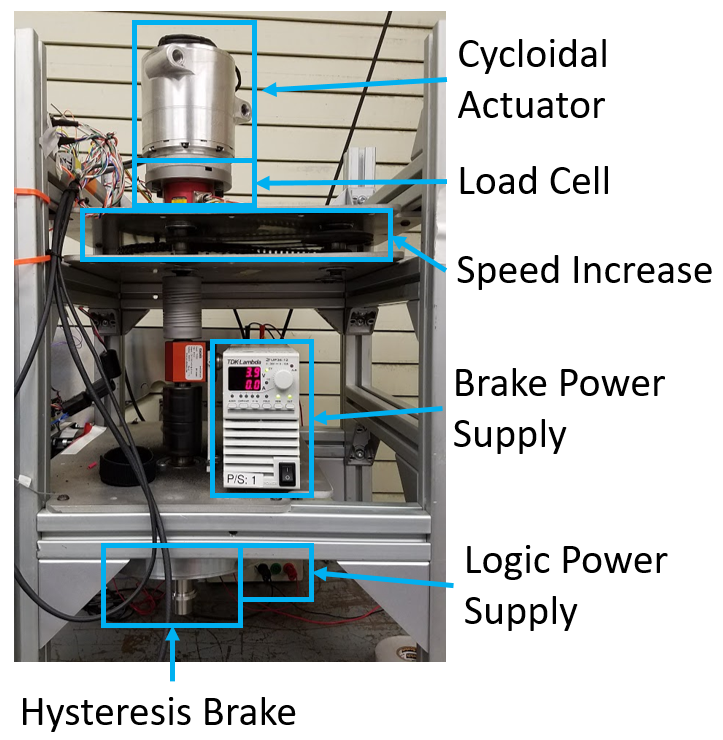
\includegraphics[width=0.75\linewidth]{fig/test_stand}
   \caption{Experimental Test Setup.
   The cycloid actuator is mounted to structure via the load cell.
   There is a speed increase so the brake can generate enough torque on the system.
   Not pictured is the controlling computer, motor driver, and high voltage supply.}
   \label{fig:test_setup}
\end{figure}

Due to the tightly integrated actuator design, the motor and cycloid cannot be separated to purely isolate the losses in the cycloid.
The efficiency map of the motor over its torque and speed range was provided by Parker Motors.
For calculation purposes, this table is used as a lookup table for efficiency of the motor given the current motor velocity and rms input current.
While this does generate a level of uncertainty in the data, these motors are mass manufactured and defects are assumed to be small.
The error in the motor efficiency map is assumed to be small and would not influence the perceived trends and results.
Power losses in the motor driver were also taken into consideration by calculating power losses in the IGBT that drives the motor.
Instantaneous current draw and a switching frequency of 12 kHz were used for the calculation, neglecting small leakage losses \cite{ref:IGBTPower}.

\begin{figure}[t]
   \centering
   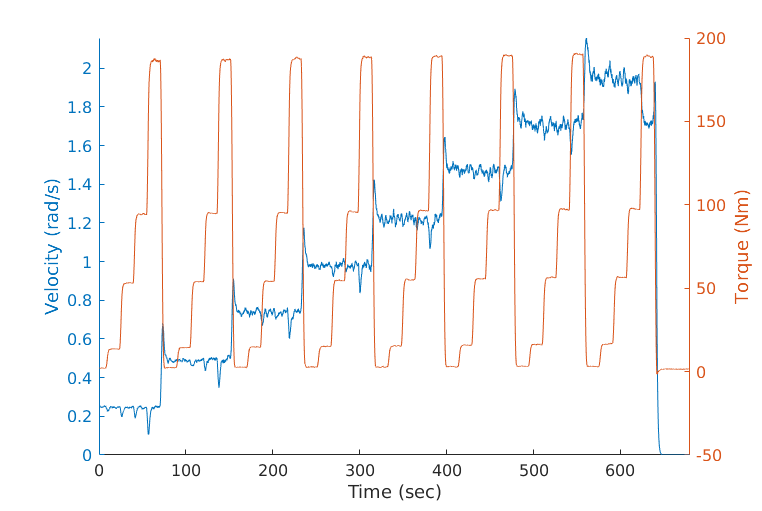
\includegraphics[width=\linewidth]{fig/eff_test_profile_v4}
   \caption{Testing profile for efficiency.
   At each speed step, torque is ramped up through five different levels, then the speed is increased.
   At the last step, the maximum of the supply was reached so motor velocity dropped.}
   \label{fig:eff_profile}
\end{figure}

The system was tested in two separate ways, an efficiency cycle and a long term drive cycle.
The efficiency cycle was run multiple times throughout the lifetime testing, first after the actuator achieved steady state efficiency, and again after each 100 hours of testing.
For the efficiency cycle, the actuator is subjected to eight velocity steps increasing 0.25 rad/s each time.
In each velocity step, the torque is ramped up and maintained for 15 seconds at values of 1Nm, 15Nm, 52Nm, 94Nm, and 189Nm.
This testing profile can be seen in Fig \ref{fig:eff_profile}.
The long term drive cycle was run continuously each day for 6 to 12 hours with the duty cycles shown in Table \ref{table:long_run}.
The total runtime of the system, not including the initial checkout and verification of the actuator, has been 303 hours.

\begin{table}[t]
  \vskip0.2cm
  \caption{Long Run Drive Cycle}
  \label{table:long_run}
  \begin{center}
    \vskip-0.2cm
    \begin{tabular}{|c||c||c|}
    \hline
    Time (s) & Velocity (rad/s) & Torque (Nm)\\
    \hline
    150 & 1.0 & 0.0\\
    \hline
    150 & -1.0 & 0.0\\
    \hline
    60 & 0.5 & 26.0\\
    \hline
    60 & -0.5 & 26.0\\
    \hline
    150 & 1.5 & 10.0\\
    \hline
    150 & -1.5 & 10.0\\
    \hline
    30 & 1.0 & 50.0\\
    \hline
    30 & -1.0 & 50.0\\
    \hline
    300 & 0.5 & 18.0\\
    \hline
    300 & -0.5 & 18.0\\
    \hline
    \end{tabular}
  \end{center}
\end{table}

It should be noted that the actuator was used briefly in the robot validation after initial development and construction of the prototype wheel module.
The total time of use was approximately three hours.
Afterwards, it was removed from the wheel module and subjected to the characterization that is discussed in this work.
The motor has a continuous current rating of 4.3 A\textsubscript{rms} and a peak rating of 15A\textsubscript{rms}.
The actuator was designed to be liquid cooled to allow operations above the continuous values, but this could not be achieved during testing.
For long duration testing, the torque values were decreased to avoid thermal issues.
The motor was tested to approximately 6A\textsubscript{rms} during efficiency testing due to the limit of the power supply.
Also, the motor driver's rated limits are 150V, therefore the actuator's maximum rated speeds could not be tested.
The nominal cycle of the actuator as seen in Table \ref{table:duty_cycle} is still achievable and has been tested.



\section{Results} \label{ch:single:eff_results}
%Discuss the results that we achieved 
% - burn in time 
% - efficiency over the current run time 
% - specific efficiency runs
% - compare to the "expected" efficiency from the rolling anlaysis 

Duty cycle testing was performed first on the actuator.
These tests were done at lower torques to prevent the motor from overheating to allow extended duration testing.
The total test time prior to these duty cycle tests was approximately 5.2 hours to bring up and check out the actuator testbed system.
Once this checkout was complete, the 300 hours of duty cycle testing were conducted over the course of 39 days with the drive cycle presented in Table \ref{table:long_run}.
Three of the torque/speed combinations in forward and reverse are plotted on Fig \ref{fig:long_run} to show the general characteristic trends seen in actuator performance.

\begin{figure}[!b]
   \centering
   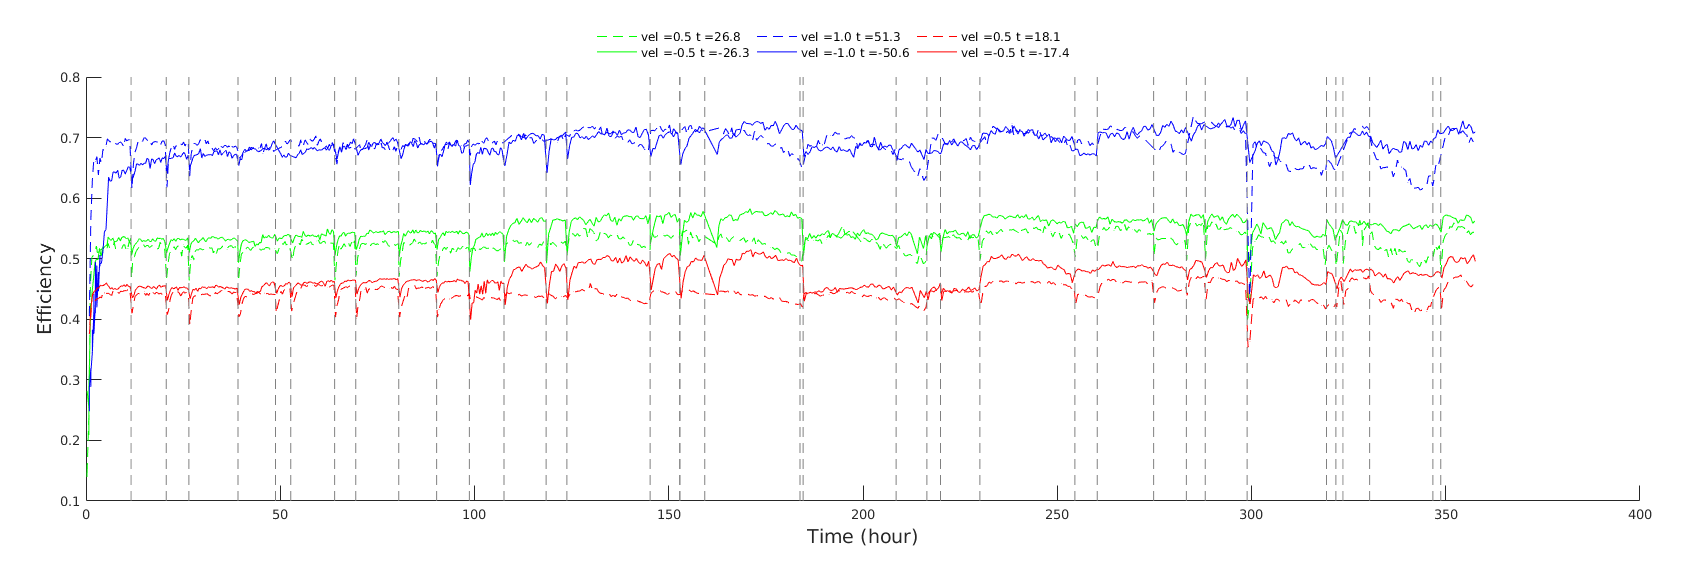
\includegraphics[width=\linewidth]{fig/total_runtime}
   \caption{Efficiency over time for three different speed/torque profiles during the drive cycle.
   The forward motion can be seen with the dotted line, reverse with the solid line.
   Testing transitions from day to day are denoted with vertical dotted lines.
   At the onset of testing, visible efficiency gains are made.
   As each day begins, there is a clear warm-up period before steady state.
   }
   \label{fig:long_run}
\end{figure}
\todo[inline]{fix the legend to be a real size}

After the break in period and steady state performance was achieved, a profile of speeds and torques (see Fig \ref{fig:eff_profile}) were run on the actuator to show the relationship between speed, torque, and efficiency.
This profile was run three times and the results at each torque and speed combination were averaged. The first efficiency cycle was run as seen in Fig \ref{fig:eff_results}. Efficiency cycles were run after each subsequent 100 hours of testing to understand performance over time. The final efficiency test is shown in Fig \ref{fig:eff_results_final}.

\begin{figure}[h]
   \centering
   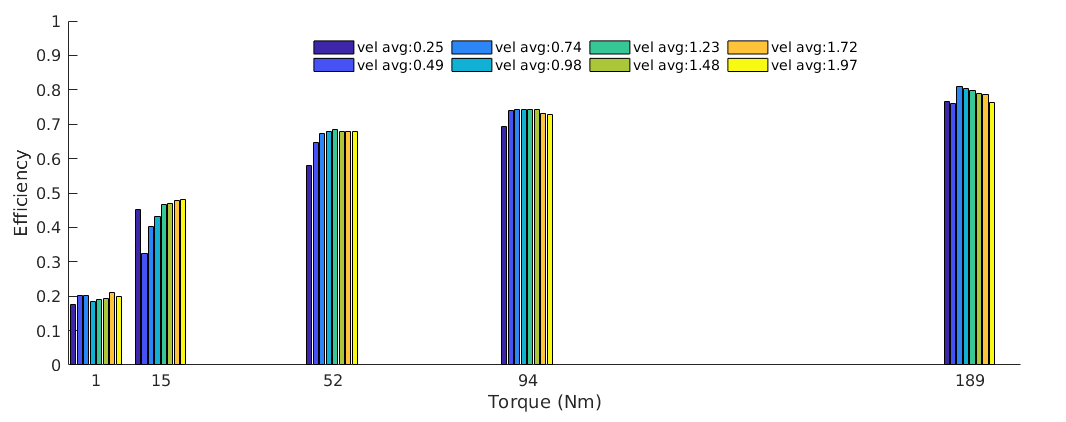
\includegraphics[width=0.8\linewidth]{fig/eff_test_bar_plot_v3}
   \caption{Efficiency of the single-stage cycloid after 100 hours of testing. Grouping of average efficiencies at each torque step.
   Efficiency depends heavily on torque, and slightly on speed.}
   \label{fig:eff_results}
\end{figure}

\begin{figure}[h]
   \centering
   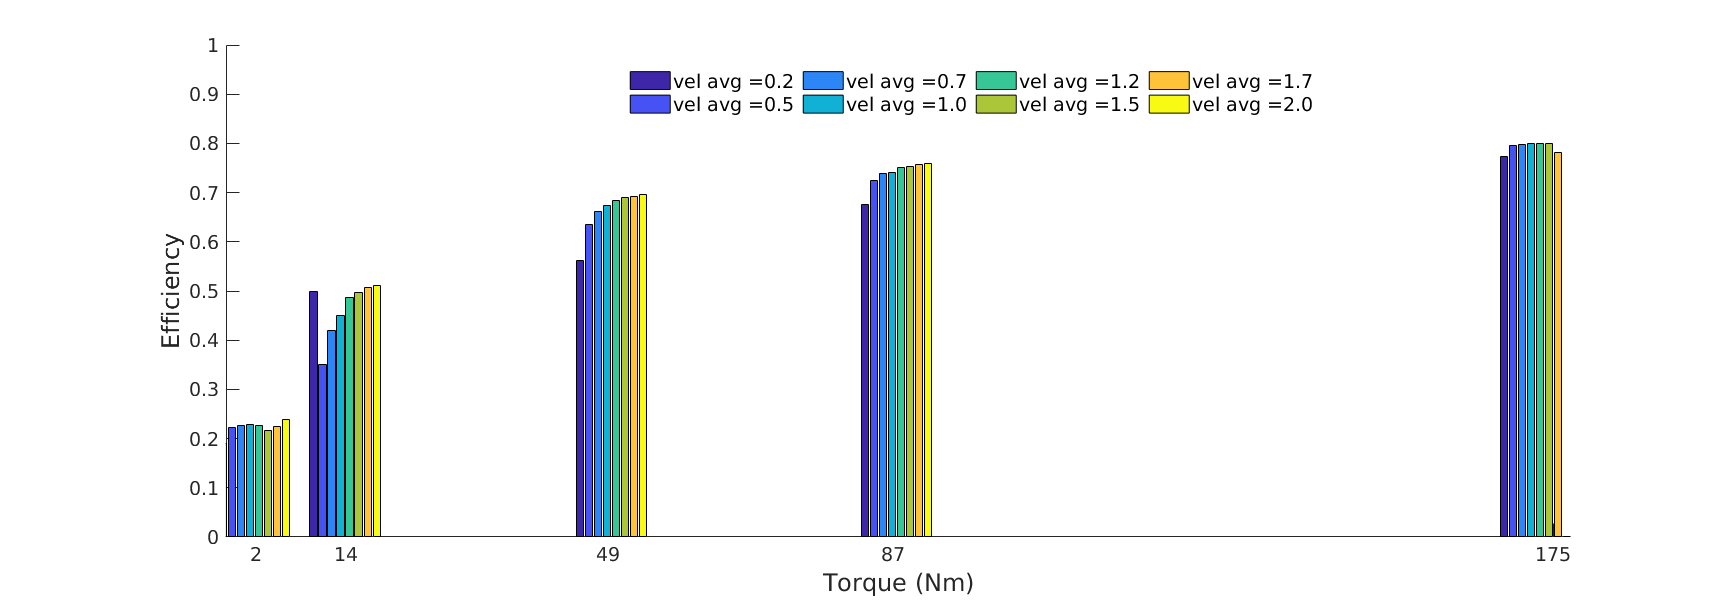
\includegraphics[width=0.8\linewidth]{fig/eff_final}
   \caption{Efficiency of single-stage cycloid after 300 hours of testing. No appreciable loss of efficiency after 129k revolutions. TODO - make the legend look the same as the one above }
   \label{fig:eff_results_final}
\end{figure}
\todo[inline]{make the legend size reasonable and the same}

\section{Wear Analysis} \label{ch:single:wear_analysis}
% Look at the pictures that we took to say "check it out, this thing can probably go for a lot longer based on how well it's done so far."
% The only real thing to look at is those plastic pieces and talk about uneven wearing on the output pins. 

After completion of the 300 hours, and 129k cycles of testing, the actuator was disassembled to qualitatively analyze the wear patterns on the cycloid. This analysis gives an interesting look as to the wear and potential lifetime of the system. 

The first note is that the grease used, Red 'N Tacky from Lucas Oil, had turned a much darker color, nearly black. The system with the output pins and plate removed can be seen in Fig \ref{fig:single_full}. After removing the individual pieces and cleaning, the wear patterns in the system become clear. The cycloid plate, Fig \ref{fig:cycloid_plate}, shows smoothing of the peaks of the lobes on the plate, where they interact with the housing pins, but shows no wear deeper in the pockets. This indicates that the machining tolerances were such that these never interacted with the pins. The wear along the faces of each lobe were consistent around the profile, suggesting each lobe carried load at some point in each cycle. Additionally, the internal holes for the output pins shows relatively even wear. These results are typical for each of the three cycloid plates. 

\begin{figure}[t]
   \centering
   \includegraphics[width=0.4\linewidth]{fig/single_full}
   \caption{The single-stage cycloid with the output plate removed. The initially red grease has been turned nearly black through operation, likely due to metal deposits from the wearing in of the system.}
   \label{fig:single_full}
\end{figure}

\begin{figure}[!b]
   \centering
   \includegraphics[width=0.8\linewidth]{fig/cycloid_plate}
   \caption{The profile of one of the cycloid plates from the single-stage actuator. Each lobe shows smoothing along convex portion of the lobe and no wear along the concave portion. The wear is also uniform around the profile, showing relatively even load distribution around the profile during operation.}
   \label{fig:cycloid_plate}
\end{figure}


Three of the housing pins can be seen as an example in Fig \ref{fig:single_housing_pins}. The wear on these pins is uniform all the way around the pin. This shows that the pin was in fact rotating in the housing during operation, as determined by the sliding analysis in Section \ref{ch:design:pin_roll_1s:sliding_equations}. These three pins are also indicative of the other 57 pins, as each had relatively uniform wear around the profile. This, coupled with the cycloid plate, suggests that during the bulk of operation, the load was shared amongst all of the lobes and pins, rather than a small set of them. This potentially could have happened during the break in period of the system as well. 

\begin{figure}[t]
   \centering
   \includegraphics[width=0.3\linewidth]{fig/housing_pins}
   \caption{The pins that rest in the housing for the single-stage cycloid. The pins showed uniform wear around their diameter and across the pins, suggesting that the load was shared relatively equally around the diameter of the actuator.}
   \label{fig:single_housing_pins}
\end{figure}


The output pins can be seen in Fig \ref{fig:single_output_pins}. The output pins were fixed in the output plate and could not roll, which is evident in their wear pattern. One side of the pin has wear, while the other still has the original black oxide coating. This result makes sense since the pin is only in contact with the cycloid plate through half of the revolution. One interesting result from this though is that some pins show much more wear than others, indicating that fewer output pins were carrying load than the maximum possible, potentially resulting in more losses. A more optimal design of this system would allow these pins to roll in their housing to wear more evenly and in a potentially lower friction interaction. 

\begin{figure}[!b]
   \centering
   \includegraphics[width=0.7\linewidth]{fig/output_pins}
   \caption{The single-stage cycloid output pins. The pins did not rotate in their housing, so the wear is uneven around the diameter of the pin. The pins also show uneven wear from pin to pin, suggesting load was not carried equally among the pins during operation.}
   \label{fig:single_output_pins}
\end{figure}

\section{Discussion} \label{ch:single:discussion}
% Summary
% single-stage reductions built in this style can result in highly competitive efficiency ratios and 2x specific torque. You still have to deal with torque ripple and a little bit of backlash (unmeasured), but if you can handle those, drop these bad boys in. 

The efficiency of the system is dependent on the torque through the gearbox as shown in Fig \ref{fig:eff_results_final}.
This contradicts previous studies that suggested that cycloidal drives have a constant efficiency across the torque range.
There is also a much less pronounced relationship between the velocity and the cycloid efficiency that can be noted in the torque bands.
This result suggests that the cycloid efficiency behaves more like a planetary or harmonic drive gearbox in its efficiency profile.
A comparison of cycloid, harmonic, and planetary efficiency profiles can be seen in Fig \ref{fig:eff_comp}.
The figure shows the efficiency for a harmonic drive CSF-45-50-2UH-LW \cite{ref:harmonic_sheet} which has a comparable ratio and torque capability to the tested cycloid and weighs 5.1kg, and a representative planetary efficiency curve from the engineers at Maxon Motor.
If backlash is acceptable in a system, a cycloidal drive can provide similar or better efficiency profiles to a harmonic drive while providing a potential 2x increase in specific torque (Nm/kg).

\begin{figure}[h]
   \centering
   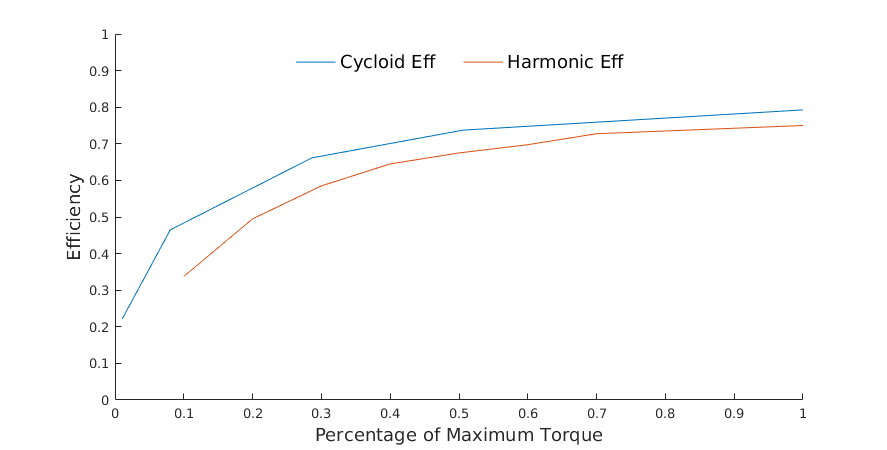
\includegraphics[width=0.7\linewidth]{fig/eff_comp_v3}
   \caption{Comparison of efficiency over maximum torque rating of the tested cycloid, a comparable harmonic drive, and a theoretical planetary gearset.
   The cycloid exhibits the same efficiency increase over torque range and has a comparable and slightly higher efficiency than the harmonic.}
   \label{fig:eff_comp}
\end{figure}

\begin{figure}[h]
   \centering
   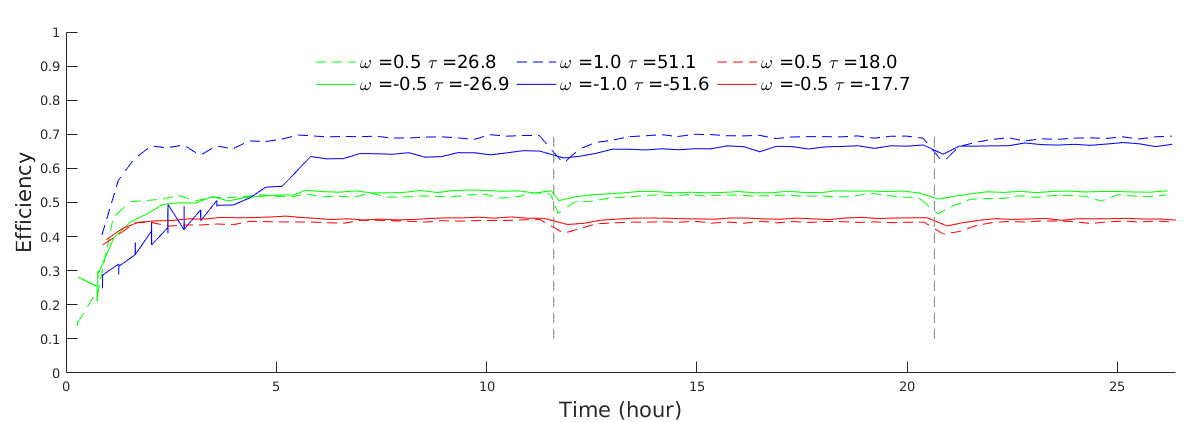
\includegraphics[width=\linewidth]{fig/burn_in}
   \caption{The first three days of testing show a substantial wear-in period for high torque periods.}
   \label{fig:break_in}
\end{figure}
\todo[inline]{fix legend size}

There was a substantial break-in time for the actuator before steady state results were achieved highlighted in Fig \ref{fig:break_in}).
In the high torque case, specifically in the reverse direction, there was an approximately linear increase in efficiency over the course of the first seven hours of duty cycle testing.
This testing began after a minimum of five hours of run time spread out through many short sessions while getting the test system running.
The large increase in efficiency can be noted in the other lower torque profiles as well, starting well below their final steady state values.
The authors theorize that this is due to break-in of the manufactured parts required because of machining inaccuracies.
Due to the complex interaction required of the trochoidal motion profile, slight manufacturing deficiencies could cause build-ups of stress and loss in particular points on the drive.
It would make sense that these could manifest in one direction and not the other if a lobe was misshapen on the trailing edge in one direction, it would be the lead in the other, causing the additional loss.
Through the first hours of testing, these materials likely wore in to each other until the contact was smooth, resulting in the more readily achieved steady state efficiencies in subsequent hours of testing.

Additionally, there is a marked improvement over the first 30 minutes of runtime in the efficiency of the system.
This is likely due to the grease and heat in the system.
The gearbox is greased with Lucas Oil Red'N'Tacky which has a viscosity index of 86 min.
This was chosen because it is designed for high loads for extended periods of time in gear and sliding surface applications, as well as ease of use for Earth testing and verification.
Therefore, during the warm-up period as the actuator temperature increases, the viscosity decrease is likely enough to cause a notable increase in efficiency of the system.
The authors leave the study of a lower viscosity grease's effect on performance, as well as grease suitable for vacuum, for future work.

Finally, through the efficiency comparison after 100 hours of testing (Fig. \ref{fig:eff_results}) and 300 hours of testing (Fig. \ref{fig:eff_results_final}) there was no appreciable loss in efficiency of the system. The actuator maintained a high level of efficiency, 81\% peak, throughout the testing. This result, coupled with the qualitative analysis of the parts after disassembly suggests that the lifetime of this actuator can greatly exceed the current testing of 129k revolutions, which suggests this is a viable actuator for robotic systems where backlash is acceptable and a high reduction and high torque actuator is necessary. 



%!TEX root = thesis_main.tex

\chapter{Design and Analysis of a two-stage Cycloid}\label{ch:dual}
% Give the abstract for a 2-stage 
% People did not put many numbers on pages for these things 
% We built one based on the available information, that lead us to understand many of the deficiencies and to further investigate, leading to the equations I'm presenting before you. 

In recent literature, new concepts have been proposed for cycloidal drives. A notable addition is a ``two-stage'' design that multiplies the cycloid reduction substantially in a very small package \cite{ref:new_two_stage}. Traditionally, a two-stage reduction takes the output of a reduction and uses it as the input of a second reduction. However, in the newly proposed ``two-stage'' cycloid, the first stage is directly coupled to the second, generating a potentially extremely large ratio in a small package. This concept is very intriguing for systems that need large reductions and have space limitations. 

With the recent advent of this style of design, there still exist many unexplored elements of the design of this drive. The kinematic layout and profile generating equations have been developed, as well as an initial development of the force calculations for one design. These are discussed in Section \ref{ch:dual:initial_equations}. Using the available literature, our group at NASA: Johnson Space Center developed a two-stage cycloid with a fused and counterbalanced set of cycloid plates (outlined in Section \ref{ch:dual:initial_equations}) and ran this actuator through a series of efficiency tests. Through these tests, gaps in the analysis of the motion and forces present in the new two-stage concept were identified, specifically pertaining to the loads and relative motion that exists in the interaction between the lobes and housing and the losses they generate. This gap is closed in the analysis of this thesis in Section \ref{ch:dual:equations}.

Through this analysis, the new two-stage cycloid is demonstrated to have potentially large efficiency losses inherent to its design. If the cycloid is designed in a similar fashion to a compact single-stage design with pins that can float in the housing, the generated forces and sliding that exists in the single-stage design is multiplied in the two-stage design, resulting in low peak efficiencies considering just the lobe to pin interaction. If a coefficient of friction of 0.03 is assumed, the peak efficiency for the as-built actuator is predicted to be 40\%. This analysis is presented in Section \ref{ch:dual:test_results} and shows that for a new two-stage cycloid to run effectively, rolling elements may need to be introduced between for the housing rollers. This is covered more in-depth discussion in Section \ref{ch:dual:discussion}.

\section{Two-Stage Cycloid Design} \label{ch:dual:initial_equations}
% Go over the 4 papers and talk about what they say, how it's derived, and finish with "what they're missing" 
% - present the way math behind my derived values, changes of frame etc. 

The traditional approach to a mutli-stage gearbox is to take the output of the reducer and use it as the input to a second reduction. In 2011, Blagojevic et. al. \cite{ref:new_two_stage} proposed a new concept for the design of a two-stage cycloid reduction in which  the first cycloid plate is connected through pins to a second cycloid plate with a different number of lobes. The housing is split between a fixed side and a side mounted to a bearing which allows rotation. The second cycloid plate interacts with the housing pins in this free-to-rotate half. The difference in number of pins, but similar motion results in potentially very large reductions. This section will first detail the motion of the system and then present the generating equations to lay the foundation for the continued analysis. 

\subsection{New Two-Stage Conceptual Design} \label{ch:dual:initial_equation:motion}

The designs presented in the initial work by Blagojevic et. al., as well as the additionally proposed design concepts by Lin et. al. \cite{ref:two_stage_tooth_mod} and Hseih and Jian \cite{ref:hsieh_effect_2016}, are predicated on the transfer of the eccentric wobble and counter-rotation of a traditional single cycloid plate to a second cycloid plate with a different number of lobes and rollers. The second set of housing pins is mounted to a bearing as the output of the system. It is the transfer of this motion from the first plate to the second plate that generates the motion to the second set of housing pins. A simple cross-section of the newly proposed concept can be seen in Figure \ref{fig:two_stage_simple_cross}. 

\begin{figure}[!b]
	\centering
	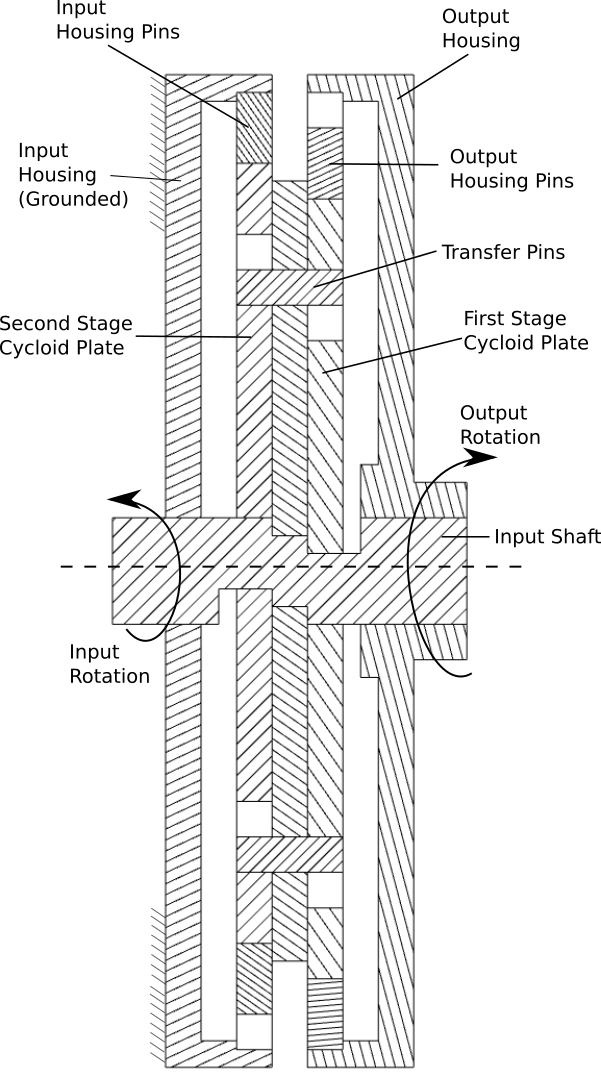
\includegraphics[width=0.48\linewidth]{fig/new_layout}
   \caption{Newly proposed layout for a two-stage cycloid. Figure adapted from Blagojevic et. al. \cite{ref:new_two_stage}}
   \label{fig:two_stage_simple_cross}
\end{figure}

The proposed designs in the literature transfer the first-stage plates counter-rotation to the second-stage plate via output rollers similar to those found in a single-stage design. These rollers then push react against a second cycloid plate that is rotated eccentrically 180$^\circ$ offset the first-stage plate to counterbalance the vibrations in the actuator \cite{ref:new_two_stage}. These elements are noted in Figure \ref{fig:two_stage_simple_cross}. The design was further developed with a rigid plate connecting the pins that transfer load from the first cycloid plate to the second, allowing increased rigidity. 

The NASA design proposes a new layout option that decreases the number of rolling elements by fusing the two cycloid plates and allowing them to rotate together rather than 180$^\circ$ out of phase. This eliminates the rolling element of the pins between the first and second cycloid plate. However, this also eliminates the natural vibration elimination, so a counterbalance must be added to the input shaft. In the design of the actuator, this weight trade between the two options was negligible, and an efficiency increase should be achieved due to the reduction of rolling elements. The assembly for this design style can be seen in Figure \ref{fig:two_stage_design}.

\begin{figure}[!b]
	\centering
	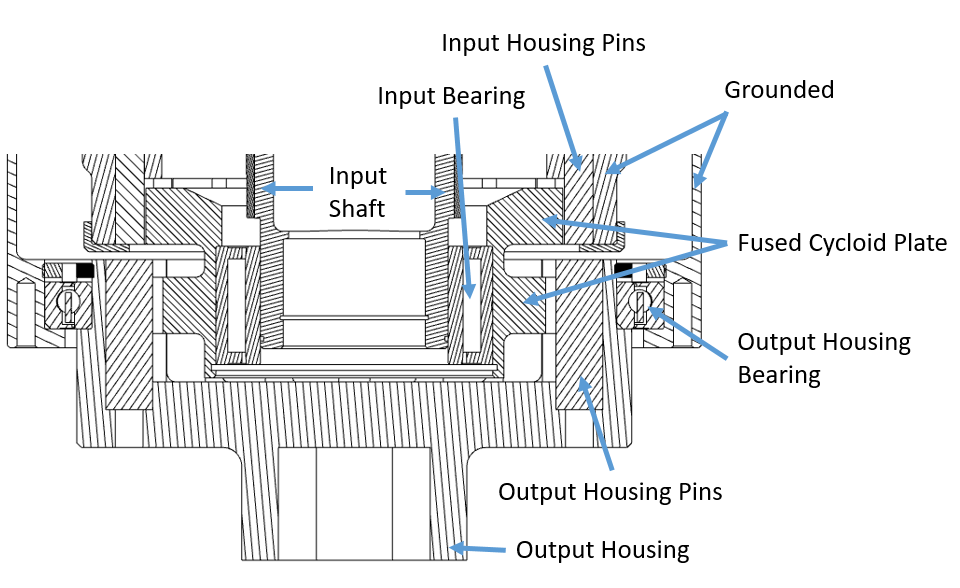
\includegraphics[width=0.70\linewidth]{fig/two_stage_cross_section_labeled}
   \caption{Cross section of the fused two-stage cycloid system designed and constructed by NASA. The counterbalance is fixed to the input shaft just above the pictured area on the figure.}
   \label{fig:two_stage_design}
\end{figure}

\subsection{New Two-Stage Profile Generation} \label{ch:dual:initial_equation:profiles}
% Go through equations that generate the profile, introduce alpha. 

To begin a design, the first thing a designer needs is the reduction of the system. This is given plainly by Lin et al. and is reproduced in Equation \ref{eq:two_stage_ratio_again}, where $N_1$ and $N_2$ are the number of housing pins for stage one and stage two, respectively.

\begin{equation} \label{eq:two_stage_ratio_again}
Q = \frac{1}{1 - \frac{N_1 (N_2-1)}{N_2 (N_1-1)}}
\end{equation}

There are two interesting items to note in this reduction equation. First, the resulting ratio is not calculated in the traditional style of ``stage-one'' multiplied by ``stage-two.'' This ``traditional'' ratio is actually only achieved in the case where the first-stage housing has one more pin than the second-stage housing. Therefore, a large gambit of ratios can be created using this style, and due to the load sharing across all of the lobes of both stages, large torque carrying capacities are possible. Second, the ratio can be positive or negative, meaning the output can spin in the same direction as the input (positive ratio) or the opposite direction (negative ratio). Due to the symmetry of the loads required, this has a very minor practical impact to the load distribution, but does result in changes in the efficiency of the system. This will be further discussed in Section \ref{ch:dual:equations}. 

\begin{figure}[t]
	\centering
	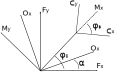
\includegraphics[width=0.50\linewidth]{fig/two_stage_frames}
   \caption{Coordinate frames used for calculating the profiles for the first and second-stage cycloid plates, as well as the resultant angles from the induced motion \textalpha.}
   \label{fig:two_stage_frame}
\end{figure}

The second step in the design process is the generation of the cycloid plate profiles. These profile equations are adapted directly from the single-stage design equations in Section \ref{ch:design:basic_calc:profile}. An addition can be made to the generating equations for the profile of the second stage that account for the motion of the output pins that will be useful for later calculations. In Figure \ref{fig:two_stage_frame}, an additional frame is added: the output frame \textit{O} relative to the fixed frame. This is the frame that the output pin rotates in with a transformation matrix. 

\begin{equation} \label{eq:T_fo}
T_f^o = \left[{\begin{array}{cccc}
		cos(\alpha) & -sin(\alpha) & 0 & 0\\
		sin(\alpha) & cos(\alpha) & 0 & 0\\
		0 & 0 & 1 & 0\\
		0 & 0 & 0 & 1 \end{array} } \right]
\end{equation}
The second stage can be generated with any desired offset from the first stage, the offset will only change the initial meshing of the output, but will have no impact on the functionality of the design. 

Using this new design concept and the basic definitions of the lobe profiles, the profiles for the two-stage design can be simply created. The positive ratio parameters laid out in Table \ref{table:two_stage_design_params} were used for the example actuator constructed and tested. Through the analysis, this will be contrasted with a design that inverts the ratio laid out in the negative ratio values.
\begin{table}[t]
  \vskip0.2cm
  \caption{Design Parameters for Manufactured Fused Two-Stage Design}
  \label{table:two_stage_design_params}
  \begin{center}
    \vskip-0.2cm
	\begin{tabular}{|c|c|c|c|}
		\hline
		Variable & Symbol & Positive Ratio Values & Negative Ratio Values\\
		\hline
		Stage 1 Housing Rollers & \textit{N\textsubscript{1}} & 19 & 18\\
		\hline
		Stage 1 Lobes & N/A & 18 & 17\\
		\hline
		Stage 2 Housing Rollers & \textit{N\textsubscript{2}} & 18 & 19\\
		\hline
		Stage 2 Lobes & N/A & 17 & 18\\
		\hline
		Total Ratio & Q & 324:1  & -323:1 \\
		\hline
		Eccentricity & $E$ & \multicolumn{2}{c|}{1.78 mm} \\
		\hline
		Roller Offset Radius & $R$& \multicolumn{2}{c|}{38.1 mm} \\
		\hline
		Housing Roller Radius & $R_r$ & \multicolumn{2}{c|}{3.79 mm} \\
		\hline
	\end{tabular}
  \end{center}
\end{table}

\section{Development of Two-Stage Design Equations} \label{ch:dual:equations}
% Go over what I have invented
% - the motion equations of the pins 
% - The load equations on the pins 
% - the projected efficiency of the system. 

After the basis of the design for the two-stage system has been laid out, more calculations are necessary for the complete design of the system. First, the force equations on the lobes will be described fully to allow for load calculations on the lobes and pins. Then, using the basis for the relative sliding velocity laid out in Section \ref{ch:design:pin_roll_1s:sliding_equations}, the relative sliding at each point will be determined. This will provide a basic estimate of loss for a two-stage cycloid system due to the interactions between the lobes and rollers. 

\subsection{Two-Stage Lobe Force Calculations} \label{ch:dual:equtions:force}

The force equations for the interaction between the lobes and rollers on the new two-stage system are initially laid out by Blagojevic et al.\cite{ref:new_two_stage}. However, these equations are for the decoupled cycloid plates. Therefore, a new set of equations is necessary for the calculation of the forces on the fused cycloid plate design. The initial equations for the derivation are presented in Section \ref{ch:design:single:force_analysis} and are based off the work by Malhorta and Parameswaran \cite{ref:malhorta_2}. 

A simple set of figures have been made to show the forces present in the fused two-stage design, yielding some interesting observations on the system. Figure \ref{fig:two_stage_force_pos} depicts the forces present in a positive ratio arrangement with an input rotation in the positive direction. The figure \ref{fig:two_stage_force_neg} depicts the forces for a negative ratio. In these two figures, it is clear that the sides the forces are acting on must flip in order to maintain the force balance. While this is an intuitive result, its physical implications for design are important. In a typical cycloid, the forces occur only on the sector that the motor's eccentric arm is on, so the forces move around with the eccentricity. Generally, cycloids are designed with machining tolerances to prevent excessive contact on the non-force sides, so contact only occurs on the eccentric side of motion. However, in the fused plate design, there is force being transmitted opposite of the eccentricity as well. Therefore, when designing in this manner, great care must be taken to ensure close meshing of the cycloid plates on all sides to limit the losses in material deflection that would otherwise need to occur to carry the load. This result also suggests that fewer than the maximum number of pins will be in contact at the same time. The study of the pins carrying load is left to future work.

\begin{figure}[t]
	\centering
	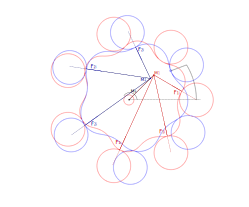
\includegraphics[width=0.80\linewidth]{fig/two_stage_loads_pos}
   \caption{Forces acting on a fused two-stage cycloid. The first-stage plate and pins are red, the second-stage plate and pins are blue. The loads on the first stage in this arrangemnt pass through the instant center for the first stage at M1. The first-stage loads are also opposite the eccentric arm, which is dissimilar from a classic single-stage ratio. The second-stage forces follow the eccentric arm through the second-stage instant center, M2. }
   \label{fig:two_stage_force_pos}
\end{figure}

\begin{figure}[t]
	\centering
	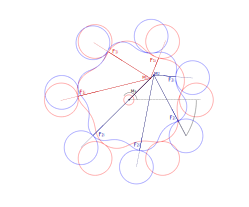
\includegraphics[width=0.80\linewidth]{fig/two_stage_loads_neg}
   \caption{Forces acting on a fused two-stage cycloid. The first-stage plate and pins are red; the second-stage plate and pins are blue. The loads on the first stage in the negative arrangement are identical to a single-stage cycloid, while the loads on the second stage are opposite the eccentric arm.}
   \label{fig:two_stage_force_neg}
\end{figure}

The next important observation from these force diagrams is that the force is acting on a different line for the first-stage and the second-stage plates. These forces act in line with the instant center that was used to generate the profile, but as noted previously, the instant center used to generate the second-stage profile is different than the instant center that is actually induced by the motion of the first stage. This phenomena will be critical fir the development of the relative motion equations in Section \ref{ch:dual:equations:vel} and the force equations in this section. 

The force calculations for the two-stage fused cycloid plate are very similar to those laid out in Section \ref{ch:design:single:force_analysis}, but instead of the balancing output forces acting on the output pins, they act on the lobes of the second stage. The forces on the first stage are denoted as \textit{F\textsubscript{1i}}, and the forces on the second stage are denoted \textit{F\textsubscript{2j}}, with an input force \textit{F}. The dimensions used for calculation for the first stage are identical to those used in a single-stage design (Equations \ref{eq:single_b} - \ref{eq:single_l}). There are only two modifications necessary to calculate these parameters for the second stage. First, \textit{N\textsubscript{1}} is substituted for \textit{N\textsubscript{2}}, and \textrho\ is calculated using the new \textit{N\textsubscript{2}}. Second, a slight modification must be made to \textbeta, as seen in Figure \ref{fig:two_stage_force_beta}. \textbeta\ must be adjusted by the output angle \textalpha. This results in the geometric values for the second stage shown in Equations \ref{eq:single_b_2} - \ref{eq:single_l_2}.

\begin{equation} \label{eq:single_b_2}
\beta_{2j} = \frac{2\pi j}{N_2} + \gamma
\end{equation}
\begin{equation} \label{eq:single_d_x_2}
d_{2x} = R \cos(\beta_j) - E N_2 \cos(\phi_2)
\end{equation}
\begin{equation} \label{eq:single_d_y_2}
d_{2y} = R\sin(\beta_j) - E N_2 \sin(\phi_2)
\end{equation}
\begin{equation} \label{eq:single_d_2}
d_2 = \sqrt{d_{2x}^2 + d_{2y}^2}
\end{equation}
\begin{equation} \label{eq:single_gamma_2}
\gamma_{2j} = \sin^{-1}\left[{\frac{R \sin{\beta_j - \phi_2}}{d_2}}\right]
\end{equation}
\begin{equation} \label{eq:single_rho2_2}
\rho_{22} = \rho_{21} - E
\end{equation}
\begin{equation} \label{eq:single_l_2}
l_{2j} = \rho_{22} \sin{\gamma_{2j}}
\end{equation}


\begin{figure}[t]
	\centering
	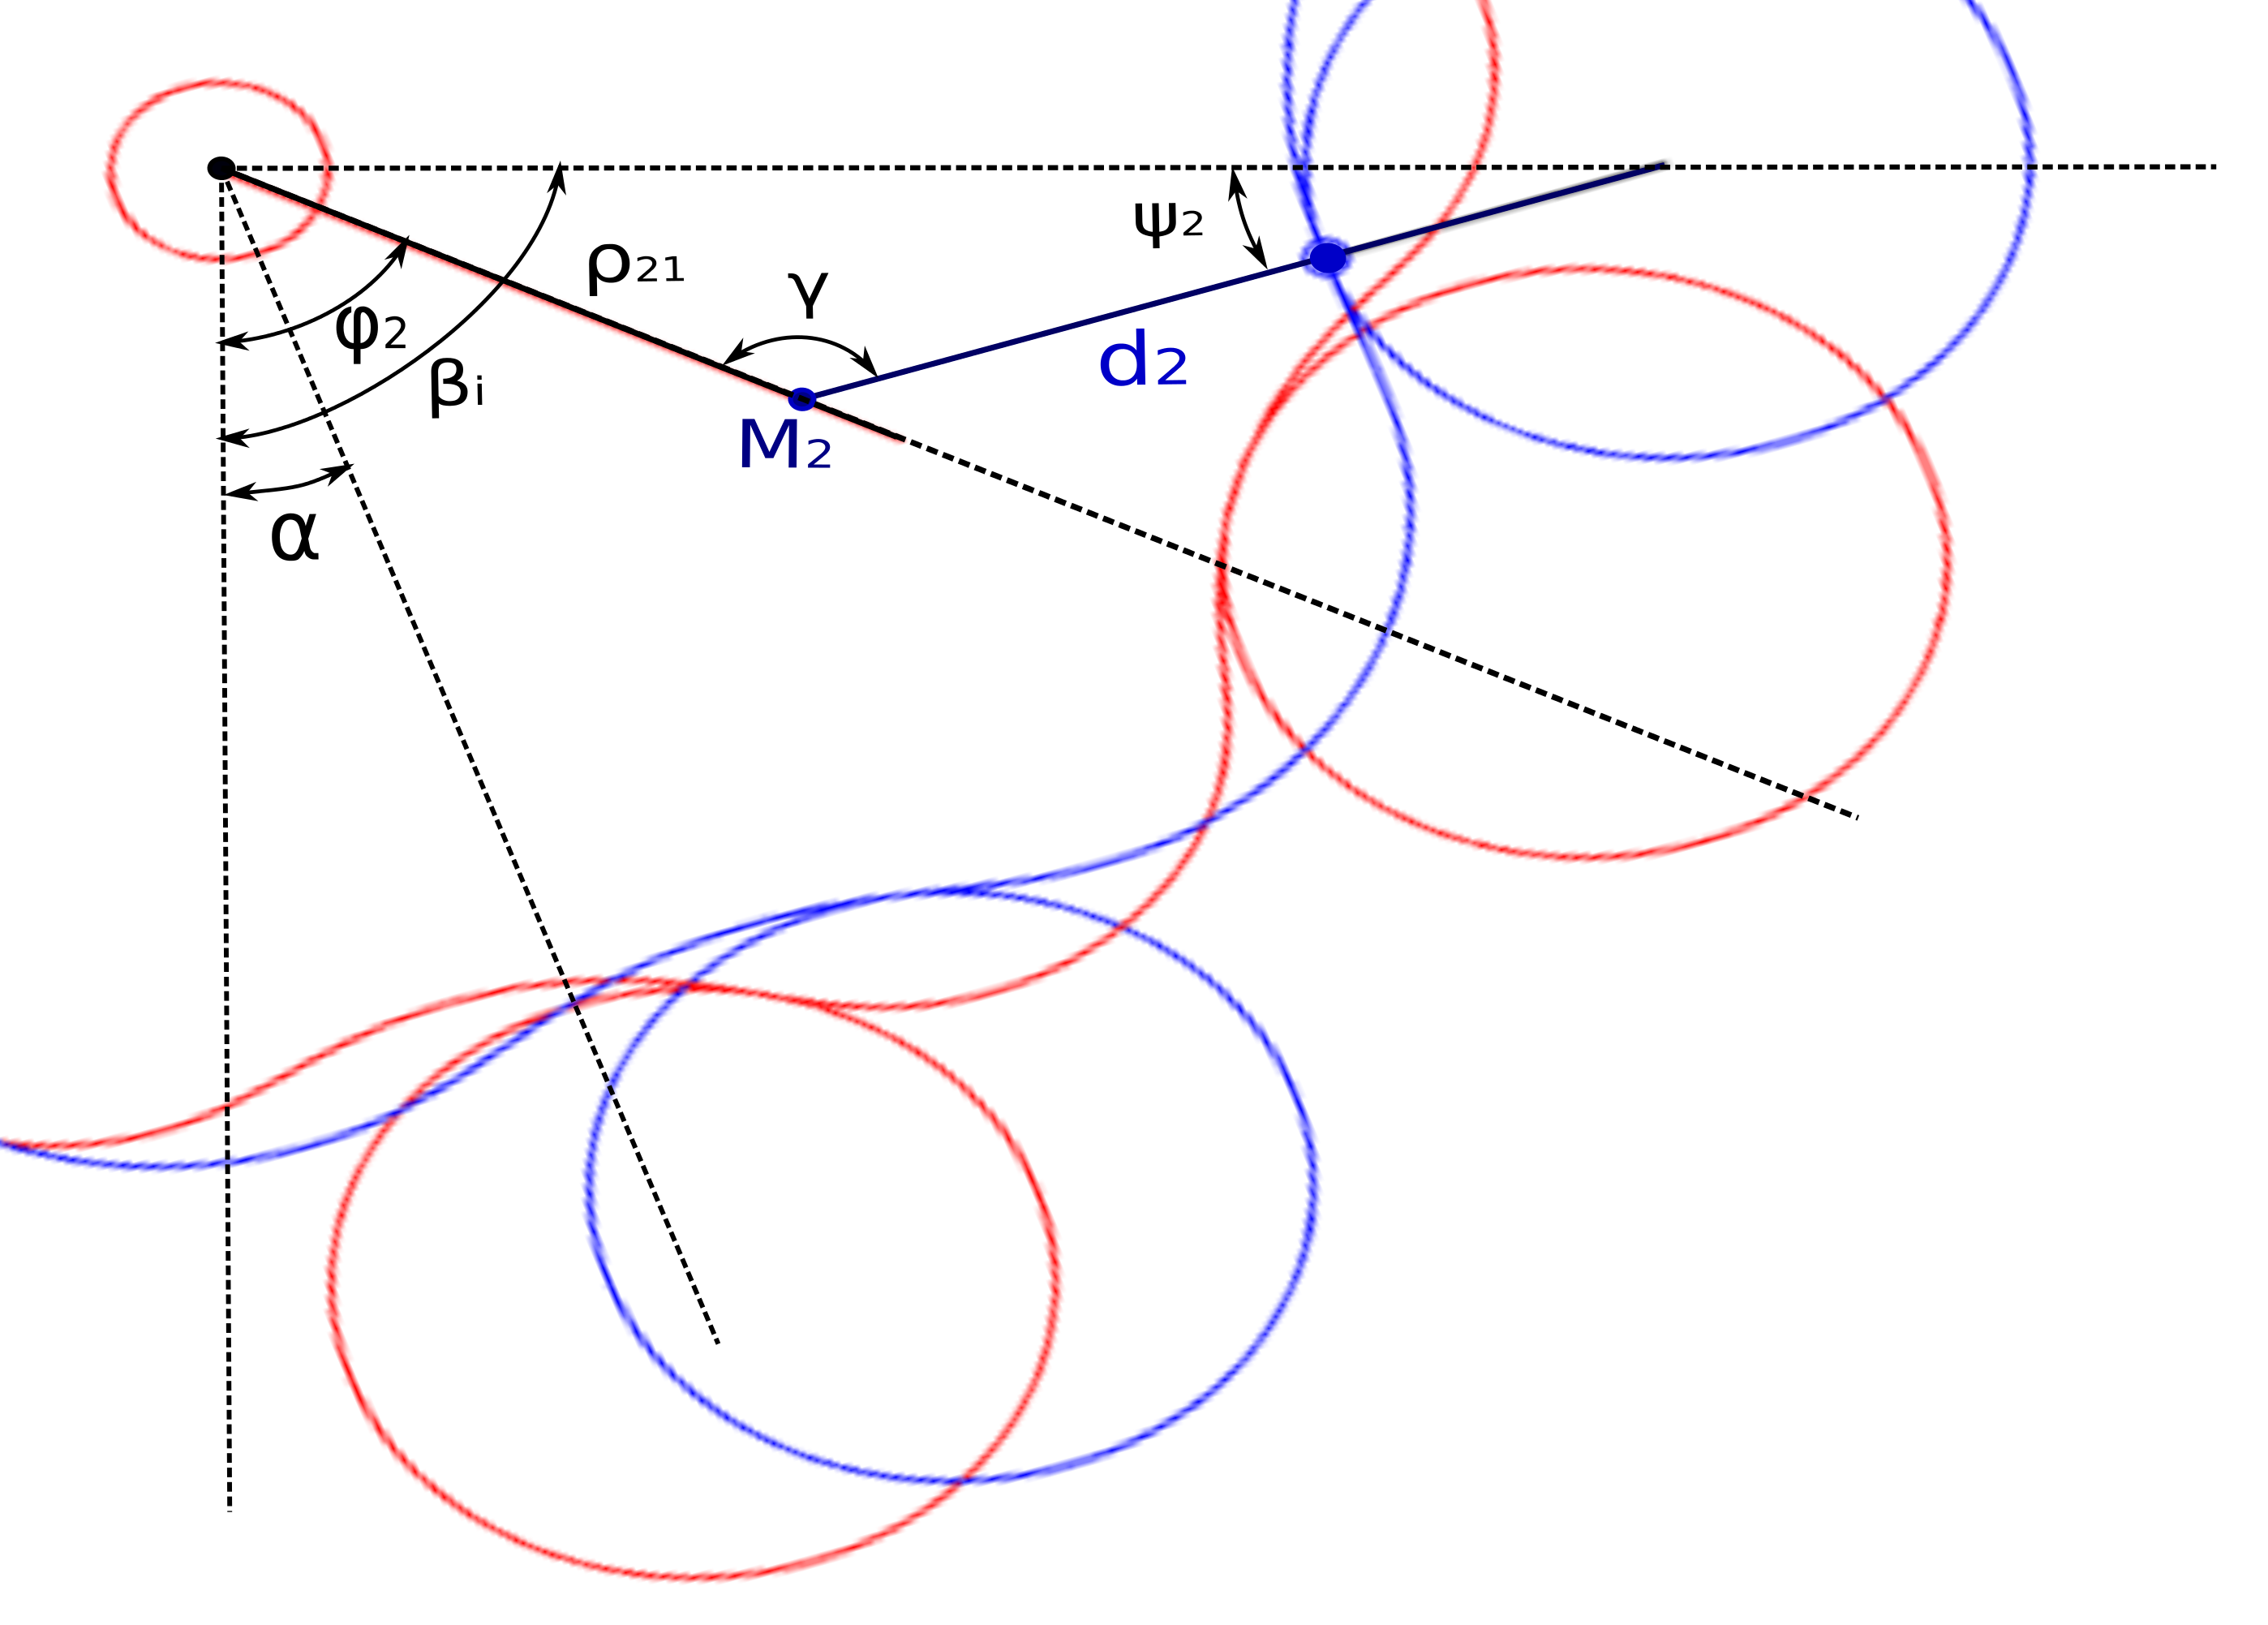
\includegraphics[width=0.8\linewidth]{fig/two_stage_loads_angles_2}
   \caption{Angles necessary for calculting the forces on the second stage of the cycloid-plate. The calculations are nearly the same as a single-stage except for a necessary modification to \textbeta\ due to the movement of \textalpha.}
   \label{fig:two_stage_force_beta}
\end{figure}

Using these design parameters and the knowledge that the number of pins in contact on the first stage, \textit{N\textsubscript{1c}}, and second stage, \textit{N\textsubscript{2c}}, are half or fewer than the total number of pins, then

\begin{equation}
N_{1c} = \frac{N_{1} - 1}{2},\ if\ (N_1 -1)\ is\ even 
\end{equation}
\begin{equation}
= \frac{(N_{1}-1) - 1}{2},\ if\ (N_{1} - 1)\ is\ odd 
\end{equation}
\begin{equation}
N_{2c} = \frac{N_{2}-1}{2},\ if\ (N_{2}-1)\ is\ even 
\end{equation}
\begin{equation}
= \frac{(N_{2}-1) - 1}{2},\ if\ (N_{2}-1)\ is\ odd 
\end{equation}

and the force equations for the first and second-stage system become

\begin{equation} \label{eq:dual_power}
M_a = \frac{R}{Q} \sum_{j=1}^{N_{2c}} F_{2j} l_{2j}
\end{equation}
\begin{equation} \label{eq:dual_torqe}
\sum_{i=1}^{N_{1c}}F_{1i} l_{1i} - \sum_{j=1}^{N_{2c}}F_{2j} l_{2j} = 0
\end{equation}

\begin{equation} 
\frac{F_{1i}}{l_{1i}} = constant 
\end{equation}
\begin{equation}
\frac{F_{2j}}{l_{2j}} = constant
\end{equation}

Using these equations, the forces on each of the lobes and pins can be obtained. The results of this analysis will be presented in Section \ref{ch:dual:test_results}.

\subsection{Lobe to Pin Contact Velocity for Two-Stage Designs}\label{ch:dual:equations:vel}
% THIS FITS INTO THE NEXT SECTION, THE QUESTION IS WHERE...
To begin to understand the losses present in the two-stage cycloid system, it is necessary to derive the sliding interactions between all of the pins and rollers, similar to the analysis initially presented in Section \ref{ch:design:pin_roll_1s:sliding_equations}.

An important distinction can be made between a single-stage cycloid and the two-stage concept used in Figure \ref{fig:two_stage_angles}. The profile for a cycloid is generated using Kennedy's Theorem, discussed in Section \ref{ch:design:basic_calc:profile}, which places the contact point between the cycloid plate and the housing roller along the straight line from the center of the housing pin to the line of centers of the motor and the cycloid plate. This distance is defined as 
\begin{equation}
D_2 = N_2 E
\end{equation} 
where \textit{N\textsubscript{2}} is the number of housing rollers in the second stage. However, because the first and second-stage plates are fused, the actual instant center of the motion of the plate must be the instant center dictated by the first-stage motion at 
\begin{equation}
D_1 = N_1 E 
\end{equation} 
defined by the number of rollers \textit{N\textsubscript{1}} in the first stage. Therefore, the same simplification that was used in the single-stage cannot be applied to both stages in the two-stage concept. 

\begin{figure}[t]
	\centering
	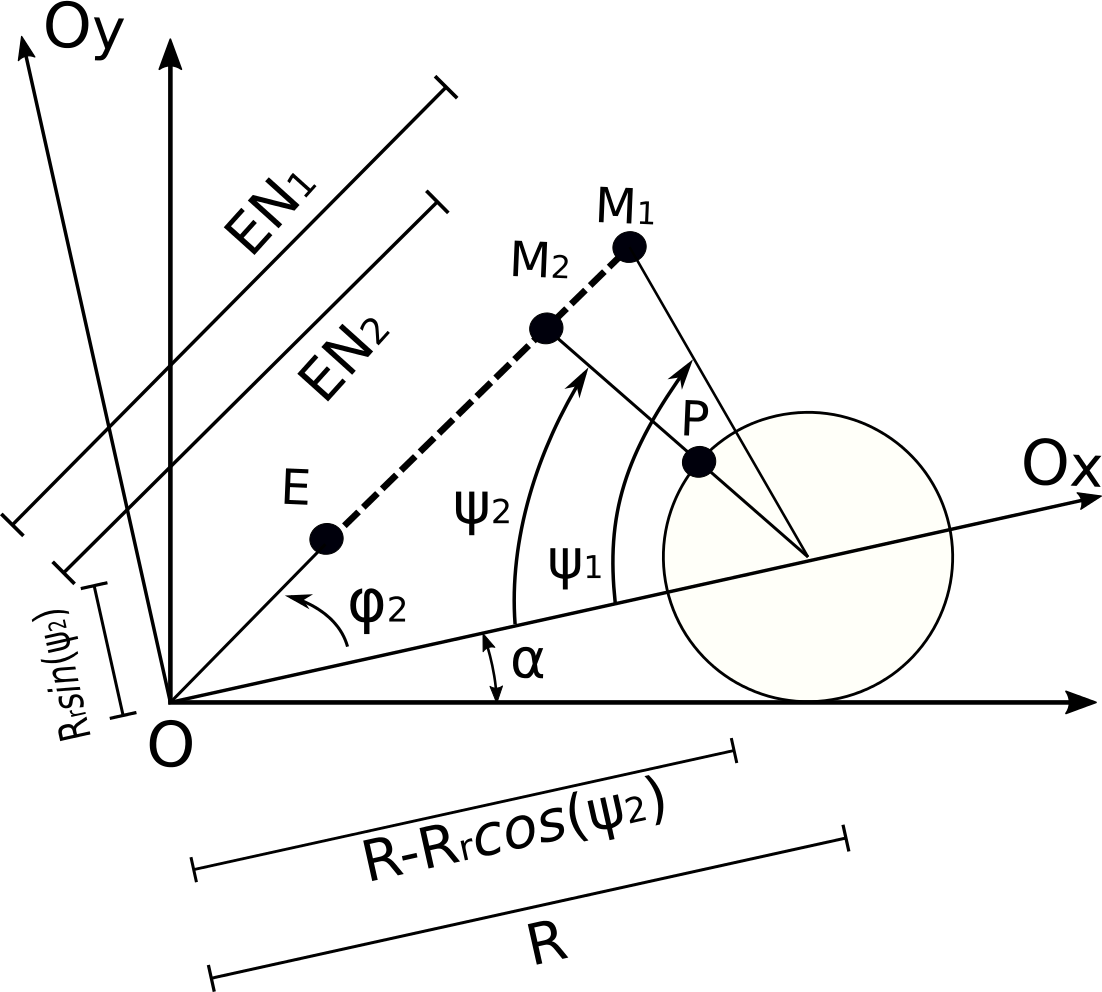
\includegraphics[width=0.50\linewidth]{fig/two_stage_angles}
   \caption{Angles for the second stage of the two-stage cycloid. The common normal through the contact point intersects at M\textsubscript{2}, creating the angle \textpsi\textsubscript{2}, but the actual instant center for the motion of the system is dictated by the first stage at \textit{M\textsubscript{1}}, defined by angle \textpsi\textsubscript{1}.}
   \label{fig:two_stage_angles}
\end{figure}


In the single-stage design, the relative velocity of the two links along the common normal, denoted as \textit{S} in Figure \ref{fig:kennedy_sliding}, is zero because the housing rollers are fixed in space. This holds true for the first stage of the two-stage concept. Therefore, the calculation of the relative velocity between the first-stage plate and first-stage housing pins is identical to a single-stage using Equations \ref{eq:single_slide_offset} - \ref{eq:single_slide_vel}. However, in the second stage of the system, the housing that holds the rollers is moving as the output of the reduction, so there is some motion along \textit{S} for the point \textit{P} located on the second-stage cycloid plate and second-stage housing rollers. Figure \ref{fig:dual_relative_motion} shows these relative velocities for the second-stage system. \textit{S} is the motion along the common normal for the point \textit{P} on both links, \textit{M} is the motion normal to \textit{S} of \textit{P} on link 1 (the second-stage cycloid plate), and \textit{L} is the motion normal to \textit{S} of \textit{P} on link 2 (the output housing rollers). 


\begin{figure}[!b]
	\centering
	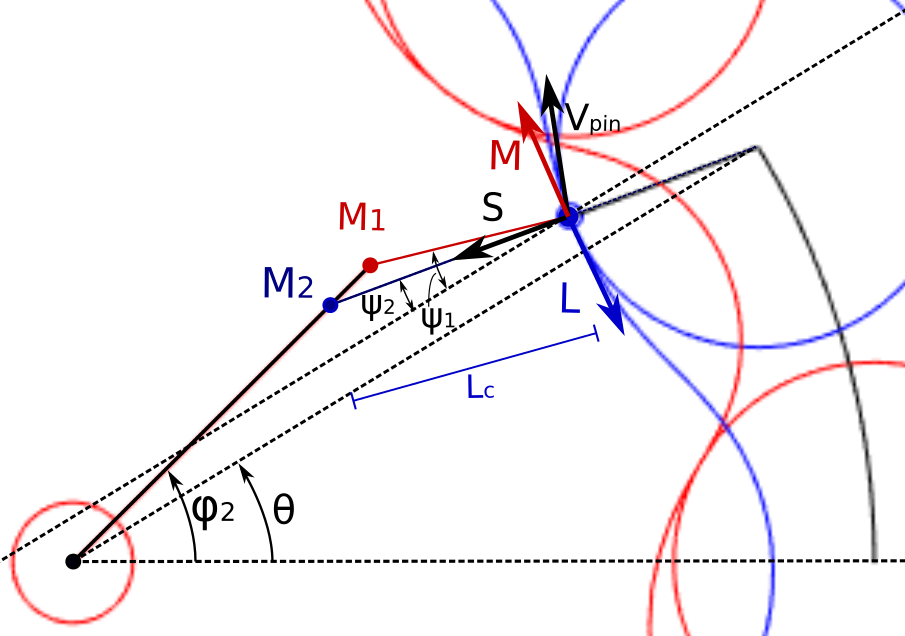
\includegraphics[width=0.70\linewidth]{fig/two_stage_vel_angles}
   \caption{Relative velocities geometric relationships. Unlike the calculations for the relative velocities of the first stage of the cycloid, the second stage has output rotation, therefore there is motion along the common normal, \textit{S}. The velocity of point \textit{P} from the output velocity of the second stage, \textit{V\textsubscript{pin}}, can be broken down into the \textit{S\textsubscript{pin}} and \textit{M}. The relative motion associated with the cycloid plate can be determined as \textit{S\textsubscript{plate}} and \textit{L}.}
   \label{fig:dual_relative_motion}
\end{figure}

First, \textit{S} and \textit{M} can be calculated for the motion of the output pins. The velocity of the output pins is the velocity of point \textit{P} induced by the rotation of the output using Figure \ref{fig:dual_relative_motion}. This velocity \textit{V\textsubscript{o}} can be defined using the output angular velocity \textomega\textsubscript{o} and the length from the concentric axis to \textit{P}, defined as \textit{L\textsubscript{op}} where \textpsi\textsubscript{2} is the angle used to calculate the profile of the second-stage cycloid plate. An angular offset, \textit{offset\textsubscript{j}}, can be applied to find the values for each pin around the ring. 

\begin{equation}\label{eq:offset2}
offset_j = j \frac{2\pi}{N_2}
\end{equation}
\begin{equation}\label{eq:psi2}
\psi_2 = \tan^{-1}\bigg\{\frac{E N_2 \sin(\phi_2-\alpha-offset_j)}{R-E N_2\cos(\phi_2-\alpha-offset_j)}\bigg\}
\end{equation}
\begin{equation} \label{eq:l_op}
L_{op} = \sqrt{(R-R_r\cos\psi_2)^2 + (R_r\sin\psi_2)^2}
\end{equation}
\begin{equation}
\gamma = \tan^{-1}\bigg\{\frac{R_r\sin\psi_2}{R-R_r\cos\psi_2}\bigg\}
\end{equation}
\begin{equation}
V_{pin} = \frac{\omega_2}{Q} L_{op}
\end{equation}
\begin{equation} \label{eq:s_pin}
S_{pin} = \frac{\omega_2}{Q} L_{op} \cos(\frac{\pi}{2}-(\psi+\gamma))
\end{equation}
\begin{equation}
V_{1} = M = \frac{\omega_2}{Q} L_{op} \sin(\frac{\pi}{2}-(\psi+\gamma))
\end{equation}


Next, the velocity along the common normal, \textit{S} and the tangential velocity \textit{L} of point \textit{P} on the cycloid plate can be determined. If the calculations are correct, the velocity \textit{S} for both the pin, \textit{S\textsubscript{pin}}, and the plate, \textit{S\textsubscript{plate}}, are equal, as they must move together to maintain contact. Figure \ref{fig:dual_relative_motion} shows the geometric values needed to calculate these relative velocities. For this calculation, the difference in angle $\psi_\Delta$ between the angle used to calculate the second-stage profile, $\psi_2$, and the angle to the instant center of motion dictated by the first stage, $\psi_1$, is calculated. Using this, the values for \textit{S} and \textit{L} are found. 

\begin{equation}\label{eq:psi_1}
\psi_1 = \tan^{-1}\bigg\{\frac{E N_1 \sin(\phi_2-\alpha-offset_j) - R_r\sin\psi_2}
{R-R_r\cos\psi_2 - E N_1\cos(\phi_2-\alpha-offset_j)}\bigg\}
\end{equation}
\begin{equation} \label{eq:psi_delta}
\psi_{\Delta} = \psi_2 - \psi_1
\end{equation}
\begin{dmath}\label{eq:L_c}
L_{c} = \bigg\{\left[E N_1 \sin(\phi_2-\alpha-offset_j) - R_r\sin\psi_2\right]^2 +
\left[R-R_r\cos\psi_2 - E N_1 \cos(\phi_2-\alpha-offset_j)\right]^{2}\bigg\}^{1/2}
\end{dmath}
\begin{equation}\label{eq:s_plate}
S_{plate} = \frac{\omega_2}{1-N_1} L_c \sin\psi_{\Delta}
\end{equation}
\begin{equation}\label{eq:L}
L = \frac{\omega_2}{1-N_1} L_c \cos\psi_{\Delta}
\end{equation}

It can be verified in the results of the analysis that \textit{S\textsubscript{pin}} and \textit{S\textsubscript{plate}} are equal, showing that the relative motion of the point \textit{P} along the common normal is in fact equal for both links, giving credence to the calculation method. Therefore, the relative velocity between the cycloid plate and the output pin can be calculated as the difference between \textit{M} and \textit{L}.

\begin{equation}
V_{2} = M - L
\end{equation}

With these equations, the relative linear sliding velocity of the cycloid plate and pins for both the first-stage and second-stage plates can be analyzed throughout the motion. These velocity results can be combined with the force results to yield the predicted losses due to this interaction in the same way as the single-stage design.

\begin{equation} \label{eq:dual_power_loss_1}
P_{L1} = \sum_{i=1}^{N_{1c}}\mu F_{1i} V_1
\end{equation}
\begin{equation} \label{eq:dual_power_loss_2}
P_{L2} = \sum_{j=1}^{N_{2c}}\mu F_2j V_2
\end{equation}


\section{Simulation and Test Results} \label{ch:dual:test_results}
% Go over the simulation results, loads in different conditions etc.
% - show the losses as a function of torque and velocity 
% - look at losses for different ratios of R/Rr 
% - show the predicted losses versus the actual losses of the designed cycloid. 

Using the equations laid out in Section \ref{ch:dual:equations}, the force and velocity on each lobe of a two-stage cycloidal drive can be calculated for a given arrangement. Using the NASA-designed cycloid as a basis for comparison, studies were run to develop the relationship between positive and negative ratio, number of pins, and coefficient of friction to develop an understanding of the optimizations available in the design, as well as compare to the ground truth of the NASA actuator. 

\subsection{Two-Stage Force and Velocity}\label{ch:dual:test_results:force_vel}
% Talk through the force and velocity on each pin. Show the graphs of the motion through space of the system. Probably can keep this short? 

The forces and velocities were calculated for the two-stage cycloid using the values set out in Table \ref{table:two_stage_design_params}. An example analysis is displayed in Figure \ref{fig:two_stage_forces_pos}. For all presented analyses, a usage scenario of 0.25rad/s output RPM and 20Nm output torque was used as a basis for comparison. Therefore, for the NASA design, an input of 0.0309Nm and an input speed of 81 rad/s was used, which given a perfectly efficient system, would yield the desired outputs. 

\begin{figure}[!t]
   \centering
   \begin{tabular}{ccc}
	   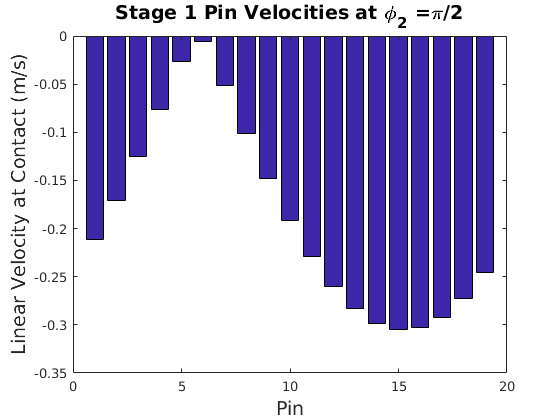
\includegraphics[width=0.50\columnwidth]{fig/double_1_vel_pi_2} &
	   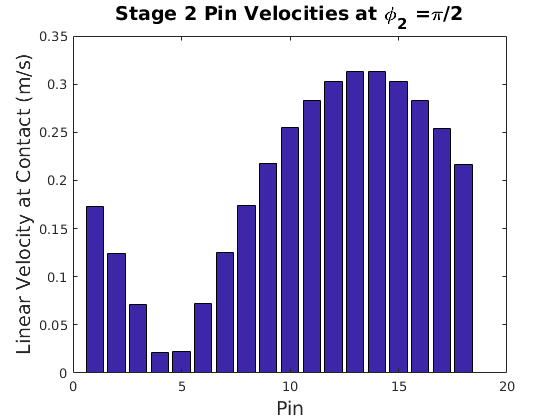
\includegraphics[width=0.50\columnwidth]{fig/double_2_vel_pi_2} \\
	   \hline
	   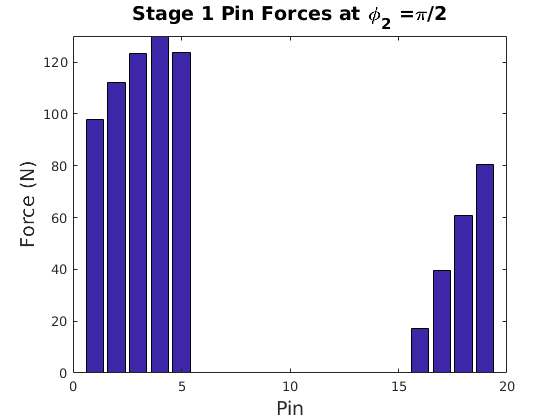
\includegraphics[width=0.50\columnwidth]{fig/double_1_forces_pi_2} &
	   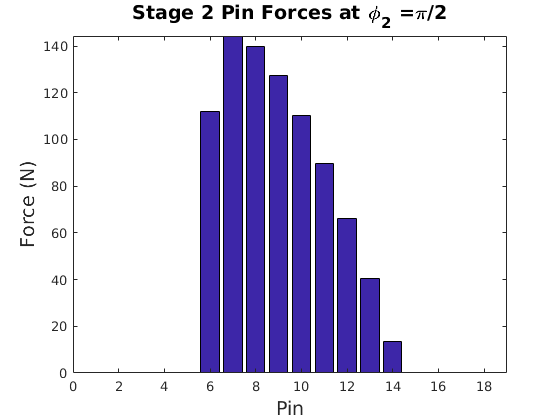
\includegraphics[width=0.50\columnwidth]{fig/double_2_forces_pi_2} \\
	   \hline
	   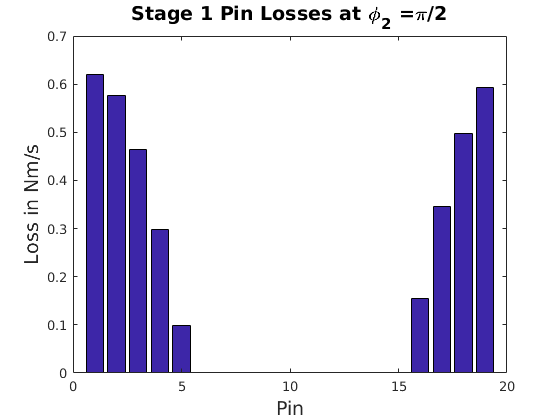
\includegraphics[width=0.50\columnwidth]{fig/double_1_losses_pi_2} &
	   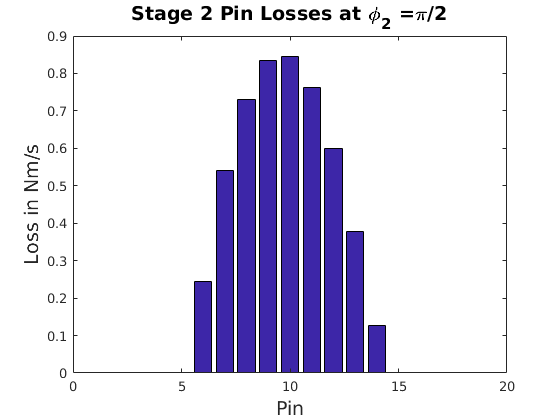
\includegraphics[width=0.50\columnwidth]{fig/double_2_losses_pi_2} \\
	   
   \end{tabular}
   \caption{Full set of velocities, forces, and losses for a two-stage cycloid system with a positive 324:1 ratio at an input angle of \textpi/2.}
   \label{fig:two_stage_forces_pos}
\end{figure}
\begin{figure}[!t]
   \centering
   \begin{tabular}{cc}
	   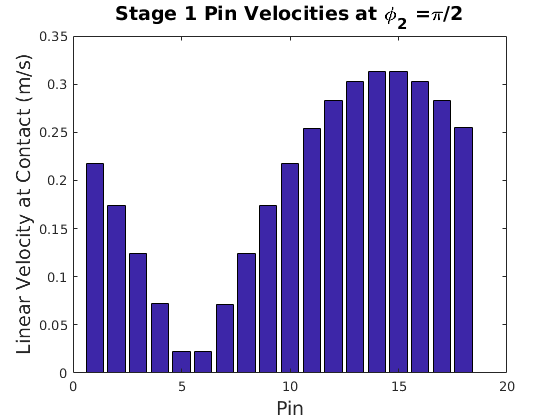
\includegraphics[width=0.50\columnwidth]{fig/double_1_neg_vel_pi_2} &
	   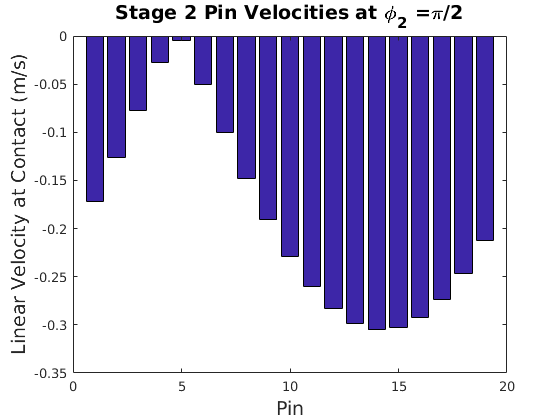
\includegraphics[width=0.50\columnwidth]{fig/double_2_neg_vel_pi_2} \\
	   
	   \hline
	   
	   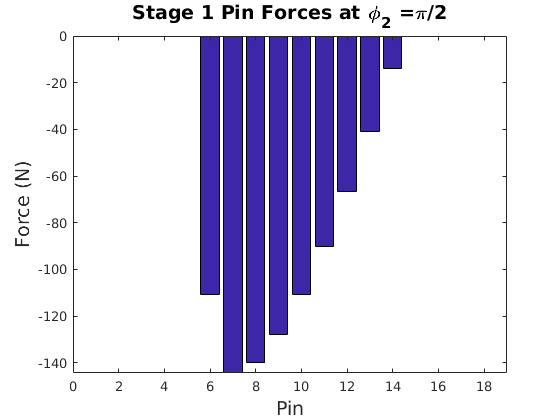
\includegraphics[width=0.50\columnwidth]{fig/double_1_neg_forces_pi_2} &
	   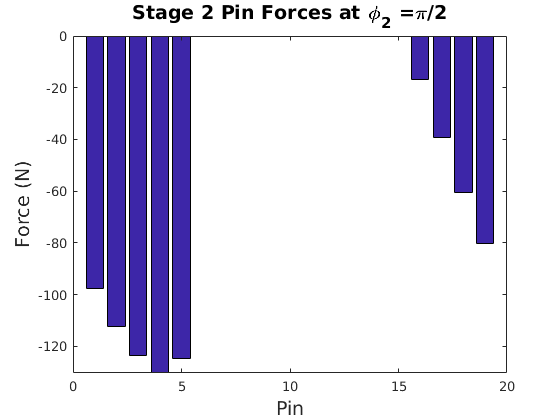
\includegraphics[width=0.50\columnwidth]{fig/double_2_neg_forces_pi_2} \\
	   
	   \hline
	   
	   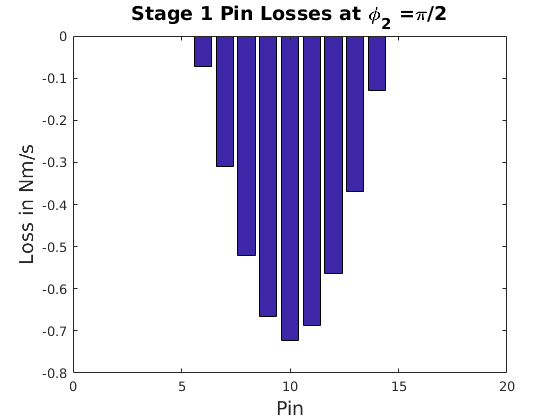
\includegraphics[width=0.50\columnwidth]{fig/double_1_neg_losses_pi_2} &
	   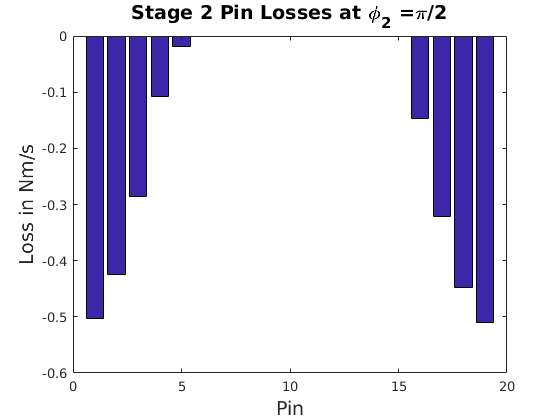
\includegraphics[width=0.50\columnwidth]{fig/double_2_neg_losses_pi_2}	\\
   \end{tabular}
   \caption{Full set of velocities, forces, and losses for the two-stage cycloid system with a negative 323:1 ratio at an input angle of \textpi/2.}
   \label{fig:two_stage_forces_neg}
\end{figure}

This can be contrasted with the similar design but utilizing a negative ratio by inverting which cycloid plate has more pins. If the first stage has more pins, the ratio will be positive; if the second stage has more pins, it will be negative. So while the parameters in Table \ref{table:two_stage_design_params} result in a ratio of 324:1, the reverse arrangement in Table \ref{table:two_stage_design_params} results in a ratio of -323:1. The same input motion simulated for the first arrangement is applied to the reverse arrangement and shown in Figure \ref{fig:two_stage_forces_neg}.

\subsection{Two-Stage Lobe to Pin Losses} \label{ch:dual:test_results:losses}
% Show the plots of the losses for the different combinations of things. Show 324 to -323, 324 - 151 - whatever, 324 to 334 

An analysis of the predicted losses for a two-stage cycloid was conducted. To determine these loss values, the forces and velocities laid out in Section \ref{ch:dual:test_results:force_vel} were used in conjunction with Equations \ref{eq:dual_power_loss_1} and \ref{eq:dual_power_loss_2} across a range of coefficients of friction to determine the losses. This result can be seen in Figure \ref{fig:two_stage_as_designed}.

\begin{figure}[t]
	\centering
	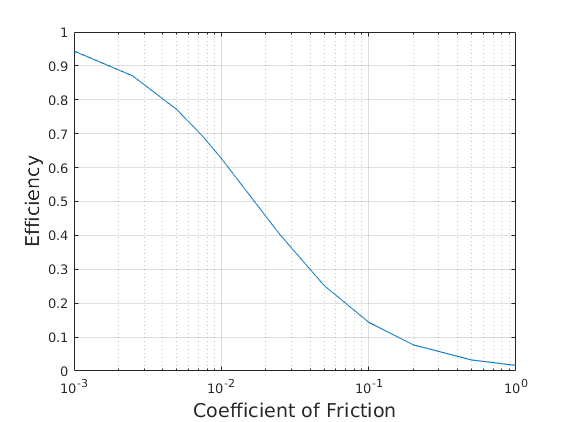
\includegraphics[width=0.75\linewidth]{fig/two_stage_as_designed}
   \caption{Predicted efficiency of the NASA two-stage cycloid for a range of coefficients of friction}
   \label{fig:two_stage_as_designed}
\end{figure}

This efficiency analysis can be contrasted against the tested values of the NASA-designed two-stage cycloid system. The constructed actuator was run through a break-in period of approximately 10 hours. During this time, the efficiency of the system was not observed to change appreciably. A test cycle, outlined in Table \ref{table:two_stage_test_cycle}, was run over the course of 10 additional hours. The testing was run using the same setup as outlined in Section \ref{ch:single:test_setup}. The two-stage was mounted in the same location as the single-stage and run with the same control equipment. The results of this cycling can be seen in Figure \ref{fig:two_stage_eff}.

\begin{table}[t]
  \vskip0.2cm
  \caption{Test Cycle for Two-Stage Cycloidal Drive}
  \label{table:two_stage_test_cycle}
  \begin{center}
    \vskip-0.2cm
    \begin{tabular}{|c||c||c|}
    \hline
    Time (s) & Output Velocity (rad/s) & Output Torque (Nm)\\
    \hline
    150 & 0.25 & 20.0\\
    \hline
    150 & -0.25 & 20.0\\
    \hline
    60 & 0.25 & 30.1\\
    \hline
    60 & -0.25 & 30.1\\
    \hline
    150 & 0.25 & 12.0\\
    \hline
    150 & -0.25 & 12.0\\
    \hline
    \end{tabular}
  \end{center}
\end{table}

\begin{figure}[!t]
	\centering
	\hspace*{-2cm}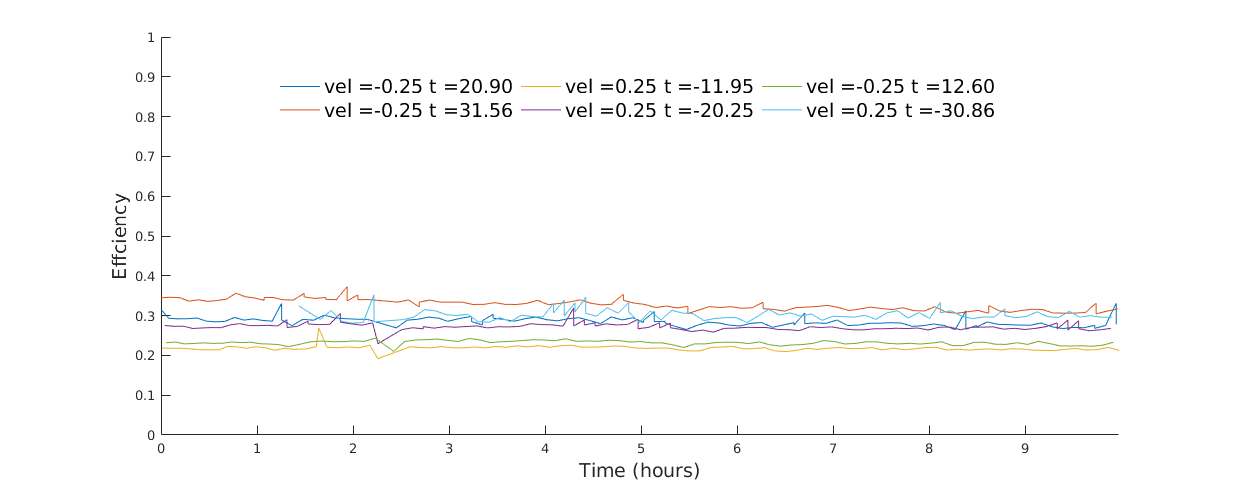
\includegraphics[width=1.2\columnwidth]{fig/two_stage_eff}
   \caption{Efficiency over time of the NASA-designed two-stage cycloid system. Each line corresponds to one of the test conditions that varied over time, outlined in Table \ref{table:two_stage_test_cycle}.}
   \label{fig:two_stage_eff}
\end{figure}

Only a modest drive cycle was run on the actuator, as its efficiencies were much lower than anticipated, therefore, the current load on the system was too high to achieve higher torques due to both over-current and over-temperature conditions of the equipment. This result is what led to the additional analysis to study the predicted losses of the system with the pin-in-housing design for a two-stage cycloid reducer. The peak efficiency observed for the cycloid was 36\%. This suggests that the coefficient of friction achieved between the rollers and housing was approximately 0.03, using Figure \ref{fig:two_stage_as_designed}. This result will be discussed in detail in Section \ref{ch:dual:discussion:actual}.


\section{Discussion} \label{ch:dual:discussion}
% Two-stages aren't awesome because you have such a multiplication of force, and the loss scales more sharply with force (not to mention the huge multiplcation of velocity too for that matter that scales by a different factor) and that causes pretty inefficient designs for this compact style. They should be built with rolling elements based on this analysis, and no one has said that yet, so boom bitches. 
% Additionally, if trying to minimize losses, you should build it negative, and you get reduced losses for more pins. 

This force and velocity analysis demonstrates a number of new and interesting revelations about the functionality of two-stage cycloids. First, the comparison between the calculated efficiencies and the achieved efficiency of the as-built actuator gives a validation to the theoretical calculations presented in this work. Next, three factors were determined to affect the efficiency of the system: the arrangement of the pins for a positive or negative ratio influences the losses in the system, the number of pins in the system influences losses, and the overall ratio influences losses. These relationships will be discussed in detail in this section. For each comparative analysis, the system was set up to yield an output torque of 20Nm and an output velocity of 0.25rad/s, similar to the testing of the built NASA reducer.

\subsection{Analysis of Pin-in-Housing Two-Stage Cycloid} \label{ch:dual:discussion:actual}

An important result stems from the comparison of the actual performance of a two-stage constructed cycloid to the theoretical calculations. For the size of the ratio desired for the design, the peak efficiency quickly falls off as the coefficient of friction increases. Coefficients of friction for lubricated steel to steel can be found from many online sources, and generally range from 0.03 to 0.15. Given this, if pins resting in the housing are used as they are in a compact single-stage design, the lowest reasonable coefficient of friction is 0.03, which makes the efficiency loss 36\% for only the interaction between the plates and pins, not including any other losses from bearing elements. The tested cycloid efficiency was shown to be in this same range. The constructed cycloid may have been achieving a nearly optimal coefficient of friction between the pins and the housing. However, even with this nearly optimal coefficient of friction, the losses are still substantial for this design. 

A generally accepted ``efficient'' system (\textless90\%) is not achieved until the coefficient of friction reaches \textless0.002, which is only achieved with roller bearings. Therefore, if a designer needs a large ratio, such as the one designed and tested, rolling elements may need to be employed at all lobe-to-pin interfaces to allow higher efficiencies to be achieved. This will substantially increase the mass and size of a two-stage system from those proposed in the literature and the one designed. However, the trade between this larger, heavier design may still lean in favor of a two-stage cycloid versus other series reductions to achieve a similar result. This mass analysis is left to future work. 

\subsection{Positive and Negative Ratio Arrangement}\label{ch:dual:discussion:pos_neg}

Other design relationships can now be analyzed using the outlined equations. The first comparison to investigate is the choice of positive or negative arrangement. The most apparent difference between the positive and negative arrangements is that the loads are flipped as the input goes around. That is, in Figure \ref{fig:two_stage_forces_pos}, the loads are on pins 1-5 and 16-19 on stage one and 6-14 on stage two, while in Figure \ref{fig:two_stage_forces_neg} this is flipped, so stage one has loads on pins 6-14 and stage tw0 has loads on pins 1-5 and 16-19. Additionally, in the positive arrangement, the load per pin is slightly lower on the first stage because there are more pins and lobes and higher on the second stage. This is reversed in the negative arrangement. 

\begin{figure}[t]
	\centering
	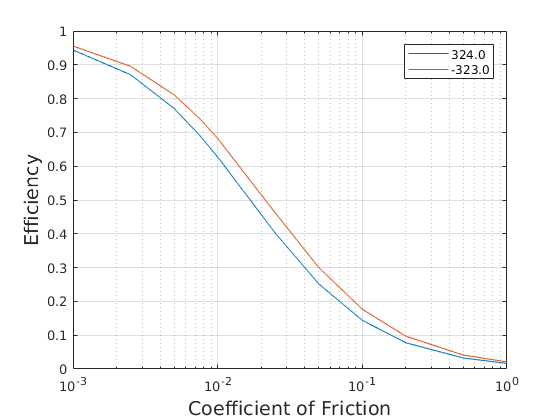
\includegraphics[width=0.75\linewidth]{fig/two_stage_pos_neg}
   \caption{Comparison of efficiencies over friction coefficients for the positive and negative ratios using the design parameters laid out in Table \ref{table:two_stage_design_params}.}
   \label{fig:two_stage_pos_neg}
\end{figure}

While these loads are simply reversed and would appear to cancel out any difference, the coupling of these loads and the relative velocities of the pins to cycloid plates plays into the predicted losses of the system, in which loss is proportional to both force and velocity. Because there is more relative motion between the cycloid plate and the pins in the second-stage plate, as evident in both Figure \ref{fig:two_stage_forces_pos} and Figure \ref{fig:two_stage_forces_neg}, if the load is higher on the second-stage plates due to this increased velocity condition, losses will increase. This relationship causes the disparity in losses for positive and negative ratios that is demonstrated in Figure \ref{fig:two_stage_pos_neg}, where the negative ratio has a lower loss per  unit of coefficient of friction. This result suggests that, whenever possible, a designer should opt for a negative ratio arrangement to decrease the losses of the actuator. 



\subsection{Number of Lobes Effect on Efficiency}\label{ch:dual:discussion:num_lobes}

\begin{table}[!t]
  \vskip0.2cm
  \caption{Design Parameters for a Similar Reduction with Nearly 3x the Number of Pins}
  \label{table:two_stage_high_pins}
  \begin{center}
    \vskip-0.2cm
	\begin{tabular}{|c|c|c|}
		\hline
		Variable & Symbol & Value\\
		\hline
		Stage 1 Housing Rollers & \textit{N\textsubscript{1}} & 51\\
		\hline
		Stage 1 Lobes & N/A & 50\\
		\hline
		Stage 2 Housing Rollers & \textit{N\textsubscript{2}} & 60\\
		\hline
		Stage 2 Lobes & N/A & 59\\
		\hline
		Total Ratio & \textit{Q} & -333.3:1 \\
		\hline
		Roller Offset & \textit{R} & 50.8mm \\
		\hline
		Roller Diameter & \textit{R\textsubscript{r}} & 1.588 mm\\
		\hline
	\end{tabular}
  \end{center}
\end{table}

\begin{figure}[!t]
	\centering
	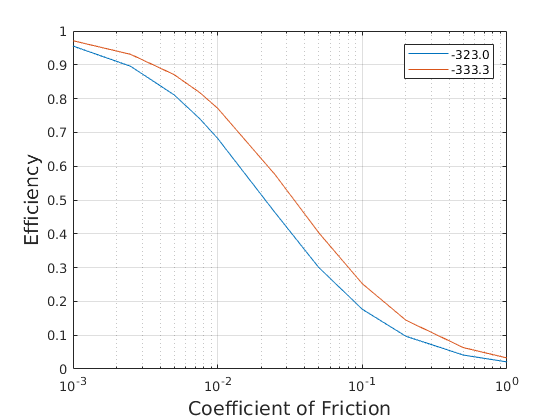
\includegraphics[width=0.64\linewidth]{fig/two_stage_more_pins}
   \caption{Comparison of the efficiencies over friction coefficient for two similar ratios, one using 18 stage 1 lobes and 19 stage 2 lobes, the second using 51 stage 1 lobes and 60 stage 2 lobes.}
   \label{fig:two_stage_more_pins}
\end{figure}

The second interesting comparison that can be done using the predicted efficiencies is the effect of the number of lobes and pins on the efficiency. The more efficient negative ratio of -323:1 was compared to a theoretical design of a -333.3:1 ratio using over twice as many pins. The design parameters for this higher pin number design were taken from the single-stage design and applied to a two-stage design. These design parameters are listed in Table \ref{table:two_stage_high_pins}. 

The theoretical efficiencies of these two systems can be seen in Figure \ref{fig:two_stage_more_pins}. This indicates that as the number of interacting pins increases, the efficiency increases. This result suggests that, where possible, a designer should use more, potentially smaller pins in a design (rather than fewer large pins) to achieve more optimal efficiencies. 



\subsection{Effect of Ratio on Efficiency} \label{ch:dual:discussion:ratio}

\begin{table}[!b]
  \vskip0.2cm
  \caption{Design Parameters for a Similar Design Using One Fewer first-stage Lobes, Resulting in ~1/2 the Ratio.}
  \label{table:two_stage_lower_ratio}
  \begin{center}
    \vskip-0.2cm
	\begin{tabular}{|c|c|c|}
		\hline
		Variable & Symbol & Value\\
		\hline
		Stage 1 Housing Rollers & \textit{N\textsubscript{1}} & 17\\
		\hline
		Stage 1 Lobes & N/A & 16\\
		\hline
		Stage 2 Housing Rollers & \textit{N\textsubscript{2}} & 19\\
		\hline
		Stage 2 Lobes & N/A & 18\\
		\hline
		Total Ratio & \textit{Q} & -152:1 \\
		\hline
		Roller Offset & \textit{R} & 38.1mm \\
		\hline
		Roller Diaeter & \textit{R\textsubscript{r}} & 3.97 mm\\
		\hline
	\end{tabular}
  \end{center}
\end{table}

The final interesting comparison completed was the effect of ratio on the efficiency. A ratio of -323:1 was compared to a ratio of -152:1, using one fewer roller and lobe on the first stage, laid out in Table \ref{table:two_stage_lower_ratio}. With the input torque and velocity scaling to achieve the same output, the predicated efficiencies are presented in Figure \ref{fig:two_stage_lower_ratio}. The result that a lower ratio results in higher efficiencies is intuitive to many designers and should not come as a surprise. This result is confirmed by this analysis. With this design, the cycloid itself would need to change very little to achieve this half ratio. The loads carried by the rollers and lobes will only increase as a ratio of the total lobes of the first ratio to the total lobes of the second ratio, because they all carry the output torque desired. The only major change in the design would be that the motor used as the input would need to double in potential torque output. This motor increase will likely lead to a gain in mass for a given design. Therefore, if optimal efficiency is more important than total mass, a lower reduction should be considered. 

\begin{figure}[!t]
	\centering
	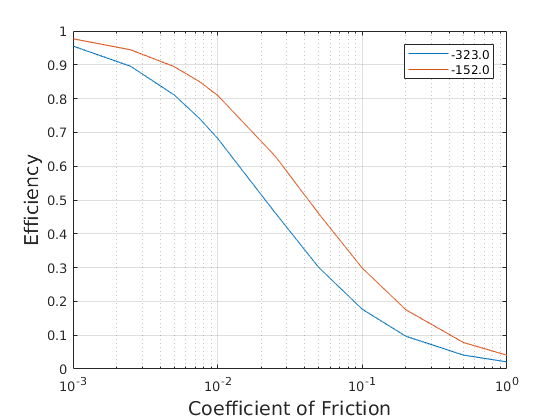
\includegraphics[width=0.75\linewidth]{fig/two_stage_lower_ratio}
   \caption{Comparison of the efficiencies over friction coefficient for two dissimilar ratios with torque and velocity inputs to achieve equal outputs. The first uses 18 stage one lobes and 19 stage two lobes, the second uses 17 stage one lobes and 19 stage two lobes}
   \label{fig:two_stage_lower_ratio}
\end{figure}

%!TEX root = thesis_main.tex

\chapter{Conclusion}\label{ch:conclusion}
% I did it I did it... Now give me my piece of paper! 

Cycloidal actuators provide the opportunity for very large reductions in a compact package with high torque capability. Cycloidal actuators are generally compared directly with harmonic drives. Compared to a harmonic drive, a cycloidal actuator can provide a 2x increase in specific torque (torque/mass). These benefits are contrasted with known deficiencies of higher torque ripple and backlash than a harmonic drive and must be traded in the actuator design. 

While the benefits of cycloidal actuators are clear and the theoretical analysis of single-stage cycloids are well documented in the literature, there are two identified gaps in the literature. The first gap is a lack of actual in-use test data, specifically for efficiency and lifetime. The second is a closed form solution of the velocity of the lobe to pin interaction and the losses associated with this interaction. 

Through this thesis, a single-stage cycloid with a 59:1 reduction utilizing the compact pin-in-housing design style was run through a series of efficiency and lifetime tests. Through the 129,000 output revolutions over the course of 300+ hours of testing, peak efficiencies of 81\% were achieved with no appreciable loss of efficiency over the testing period. Additionally, it was demonstrated that a substantial break in period of 10+ hours may be necessary before steady state efficiencies are achieved. The compact single-stage cycloid tested had a 2x increase in specific torque over a harmonic drive rated for the same loads and speeds and achieved slightly higher efficiencies than published in the harmonic drive data sheets. If backlash and torque-ripple are acceptable in design, a compact cycloid is a valid design choice. Additionally, the closed form equations for the relative velocity between the cycloid plate and housing pins/rollers were developed and demonstrated. An analysis was conducted to compare to the tested cycloid. This analysis supported the results of the efficiency testing of the single-stage design.
% mention the relative motion analysis

A new addition to the literature within the last few years is the concept of a compact two-stage cycloid design in which the motion of the first stage cycloid plate is used to directly drive the motion of the second stage cycloid plate. The second stage plate drives the second stage pins to achieve very large potential reductions. The kinematics for this design have been presented in the literature with brief analyses of the loads expected on the cycloid plates. 

A two-stage cycloid was designed and tested using these kinematic equations, and a gap was identified in the analysis of these two-stage systems, resulting in large inefficiencies of the design. Therefore, analysis was done to study the interaction between the forces and velocities at the lobe-pin interaction and predict the efficiency losses associated with this interaction. This work demonstrates that the losses associated with the as-built design for a compact pin-in-housing design result in best-case efficiencies of ~36\%, suggesting that high ratio designs must utilize rolling elements for these interactions to achieve acceptable efficiencies. Additionally, comparisons were done to give guidelines for designers. A two-stage cycloid with a negative ratio arrangement results in increased efficiency for a given coefficient of friction for the pin to housing interaction. A design utilizing more pins also results in a higher efficiency. Finally, a lower ratio with similar outputs can result in higher efficiencies. 

Overall, this work has demonstrated that a single-stage cycloid is a valid design choice in robotic actuators. If backlash and torque-ripple are acceptable, a single-stage, pin-in-housing design can achieve higher efficiencies than a harmonic drive with a reasonable expected lifetime and half the mass. In addition, this work contributes additional necessary design equations for the sizing and design of a two-stage cycloid system. Further experimental testing will need to be done to validate the losses of a bearing-in-housing design of this system. 


%Currently, harmonic drives are the primary speed reducer for robotic applications where a high reduction in a small package is required. 
Cycloidal drives are an alternative option for high reduction, small package, use-cases with the advantage of a higher specific torque and the ability to customize and integrate the drive for the application.
These compact style cycloidal drives have been well studied in theory and simulation for their performance, but very little data is available on their actual performance over time. 
This paper presents experimental data on performance of a cycloidal drive designed for a robotic application. 
Burn-in time efficiency curves and torque/speed efficiency profiles are computed after running the drive through 51k output cycles (3M input cycles) over the course of 111 hours of testing. 
The study finds that substantial burn-in time may be required for steady-state performance, but peak efficiencies of 81\% can be achieved. 
Also, the efficiency is shown to be dependant on the torque through the actuator.
This work demonstrates a customized cycloidal drive in a robotic application that is comparable to a harmonic drive in efficiency performance, with a 2x increase in specific torque, suggesting the application of cycloidal drives could grow tremendously in robotic designs. 
%As robotic applications flourish in our modern world, there is an increasing need for high reduction, high torque, and low backlash actuator systems.
These actuators are present in all types of robotic equipment and are critical in space flight applications.
A notable recent example includes the Curiosity rover from NASA's Jet Propulsion Laboratory that uses 33 separate motors with various reductions \cite{ref:curiosity}.
Currently, harmonic drives are the primary reduction method when high ratio and compact design are required.
Commercially, these reducers come in limited reduction ratio options, and require a substantial amount of additional mass to withstand high torque applications.
Ideally, one would be able to specify a desired reduction ratio and realize it in a compact, lightweight package.

\subsection{Cycloidal Drive Motivation}

Cycloidal drives are potentially an apt replacement for these harmonic drives as they can offer large a large reduction in a small package.
In situations where small backlash is acceptable, cycloids offer distinct advantages.

\begin{enumerate}
\item
They can be customized into the system directly. They allow specific reductions and load selection and can be incorporated directly into the actuator housing.
\item
They are made of relatively easy to manufacture parts.
\item
The torque to weight ratio typically higher for cycloidal drives of this style.
For example, the cycloid presented in this work is 2.5kg including all housing components, while a comparable harmonic drive is 5.1kg.
\end{enumerate}

Cycloidal drives have many desirable characteristics, but are not commonly used in robotic actuator design due to the lack of data that is available about their operation.

The primary contribution of this research is to quantify the efficiency of a cycloidal drive system through an extended drive cycle test for burn-in to steady state performance and efficiency over the torque/speed profile.
To date, the actuator has been subjected to over 51k output revolutions through over 100 hours.

\begin{figure}[!b]
   \centering
   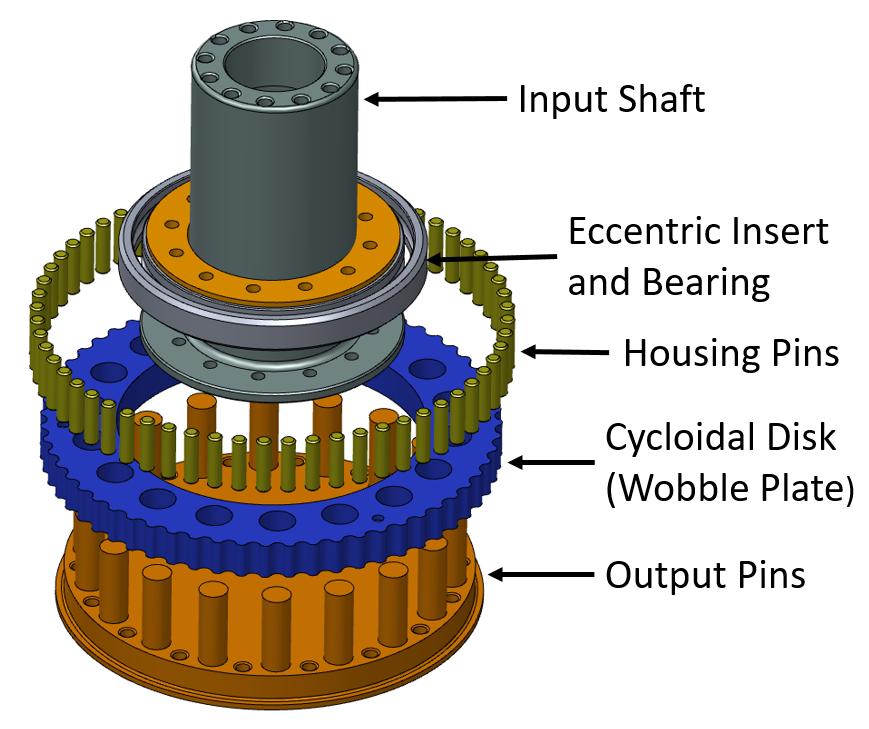
\includegraphics[width=0.60\linewidth]{fig/cycloid_cartoon_v2}
   \caption{Simple rendering of the key elements that create a cycloidal drive.
   A drive shaft spins a cycloidal disk (wobble plate) via an eccentric circle.
   The wobble plate reacts against the housing pins to create a counter-rotation, harnessed by the output pins.}
   \label{cycloid_cartoon}
\end{figure}

\subsection{Cycloidal Drive Background}
Cycloidal drives were proposed as early as 1956 by Botsiber and Kingston \cite{ref:1956}.
The premise of this design leverages a plate, referred to as the wobble plate, with lobes interacting with pins in the housing designed using trochoidal motion being spun on an eccentric shaft with a bearing.
This eccentric lobe to pin interaction induces a counter-clockwise motion of the plate that is harnessed with the interior pins as the output of the mechanism (seen in Fig \ref{cycloid_cartoon}).
This geartrain design has been used in industry for high torque, high shock load applications for many years including companies like Natbesco Motion Control.
However, in many of these applications, many or all of the interacting surfaces like the housing pins and output pins use needle roller bearings to transmit load.
This allows for higher efficiency and load carrying capability, but it also increases mass and volume.
In the robotic industry, groups are striving to reduce the mass and volume of these actuators while still achieving high reduction and load capabilities.
One method for reducing mass is eliminating the rolling elements at the interaction points between the wobble plate, housing pins, and output pins.
This allows for very compact and strong designs to be considered, but leaves the potential for larger losses and shorter system lifetime.

Many works have been presented on the subject of the theoretical design of these cycloidal drives \cite{ref:on_the_lobe} \cite{ref:hwang_hsieh}, designing with machine tolerances \cite{ref:design_and_application}, contact and stress analysis \cite{ref:li}, and performance characteristics such as torque ripple and backlash \cite{ref:hsieh_traditional} \cite{ref:hsieh_dynamics} as will be presented in Section \ref{design}.
These works lay a solid foundation for a designer, providing the equations and design considerations for a cycloid.
Still, there is a need to present in-use characteristics to support the theoretical calculations and models.

Theoretical cycloid efficiencies have been reported in the 88-98\% range \cite{ref:Malhorta}, \cite{ref:unified_approach}.
More recently, Sinsinger and Lipsey reported experimentally determined efficiencies for fused roller designs (42.3\%) and pin designs (71\%) based on 80 minutes of run-time \cite{ref:cycloid_vs_harmonic}.
The distinction between a fused roller and pin design comes in the design of the housing.
In a fused design, the input pins are machined as part of the housing, and in a pin design, pins are inserted to ride in the housing, allowing relative motion.

Hsieh verified the stress present in the drives in simulation and in-use which demonstrated lower stress levels and torque ripple when using fused rollers \cite{ref:hsieh_dynamics}.
These two results leave an open trade to designers if stress and torque ripple need to be minimized versus maximizing efficiency.

The aim of this work is to utilize a custom cycloid design for a NASA rover application and show the in-use efficiency characteristics over an extended duration test.
The actuator design is presented in Section \ref{design}.
A description of the experimental setup and procedure is provided in Section \ref{methods}.
Finally, the results and analysis of this high torque actuator and its implications are presented and discussed in Section \ref{results} and Section \ref{discussion}.


%\begin{table*}[t]
  \vskip0.2cm
  \caption{Designed Duty Cycles for System}
  \label{duty_cycle}
  \begin{center}
    \vskip-0.2cm
    \begin{tabular}{|c||c||c| |c| |c|}
    \hline
    Time Used & Output Torque (Nm) & Output Speed (RPM) & Actuator Torque (Nm) & Actuator Speed (RPM)\\
    \hline
    5\% & 2440 & 6.8 & 554.7 & 33.9\\
    \hline
    20\% & 1627 & 6.8 & 369.8 & 33.9\\
    \hline
    60\% & 542 & 15.3 & 123.3 & 76.3\\
    \hline
    15\% & 135 & 15.3 & 30.8 & 76.3\\
    \hline
    \end{tabular}
  \end{center}
\end{table*}

In 2007 and 2008, NASA developed a manned rover prototype for planetary surfaces for future missions \cite{ref:rover}.
This robotic vehicle is made up of six independent wheel modules, each with their own drive, steering, and both active and passive suspension.
In 2014, a new prototype wheel module was designed and created to analyze potential technologies that could be used in these applications.
In the new design layout, it was possible for the drive wheels to counter-rotate against the steering and put large shock loads into the steering system.
These requirements called for a compact package, high load, high shock load, and tolerance of backlash lent themselves to the selection of a cycloidal drive for the steering actuator.
The prototype wheel module layout can be seen in Fig \ref{wheel_module}.

\begin{figure}[t]
   \centering
   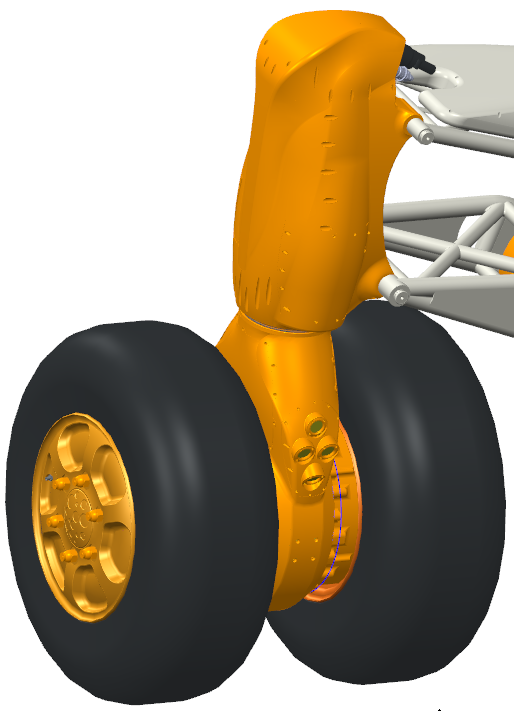
\includegraphics[width=0.40\linewidth]{fig/wheel_module_CAD}
   \caption{CAD model of rover wheel module prototype.
   Suspension arms hold the steering column.
   Each wheel has an in-wheel drive motor.}
   \label{wheel_module}
\end{figure}

Based on the load cases, the actuator was required to output a stall torque of 2,440 Nm (1800 ft-lb) with a max output speed of 1.57 rad/s (90 deg/s) at 1,626 Nm (1200 ft-lb).
The required torque/speed data points are presented in Table \ref{duty_cycle} with an assumed loss of 88\% chosen based on the available literature.
The actuator layout for the vehicle placed the motor and cycloid off center of the steering axis with an additional 5:1 reduction into the steering column, thus decreasing the torque needed for the cycloid output, but increasing the potential shock loading.

Many sources have laid out the design parameters for these drives and the equations are provided below for completeness.
Shin and Kwon \cite{ref:on_the_lobe} presented the mathematical definition of the cycloid profile as

\begin{equation} \label{eq:0}
Z = \frac{Z_1} {Z_2 - Z_1}
\end{equation}
\begin{equation} \label{eq:1}
C_x = R cos\phi -R_r cos(\phi + \psi) - e cos((Z_1 + 1)\phi) 
\end{equation}
\begin{equation} \label{eq:2}
C_y = -R sin\phi + R_r sin(\phi + \psi) + e sin((Z_1 + 1)\phi) 
\end{equation}
\begin{equation} \label{eq:3}
\psi = tan^{-1} \lbrack\frac{sin(Z \phi)}{cos(Z \phi) - R / (e(Z + 1))}\rbrack 
\end{equation}

where \textit{Z} is the overall reduction, \textit{Z\textsubscript{1}} is the number of lobes, \textit{Z\textsubscript{2}} is the number of pins, \textit{R} is the distance from the center to the rollers, \textit{R\textsubscript{r}} is the diameter of the pins, \textphi\ is the angle of the input shaft and \textpsi\ is the angle of contact between the outer pin and the cycloid lobe.

Using both the formula for the reduction in diameter of the cycloid disk to account for machine tolerances \cite{ref:machine_design} \cite{ref:design_and_application} as well as Ye et al.'s formula for calculating the limit of undercutting \cite{ref:ye}, the allowable sizes of the profiles and pins can be determined.
Sensinger \cite{ref:unified_approach} laid out simple equations for calculating stress on the lobes and pins that has been further modelled and studied by others.
The force on the cam for calculating the bearing load with eccentricity e, ratio Z , and torque T is

\begin{equation} \label{eq:4}
F_{cam} = \frac{T}{e Z}.
\end{equation}

The simplified stress equations where \textit{t} is the contact thickness, and \textit{b} is the width of contact determined by (\ref{eq:7}) and (\ref{eq:8}) are

\begin{equation} \label{eq:5}
F = \frac{T}{R - R_r}
\end{equation}
\begin{equation} \label{eq:6}
\sigma = \frac{2F}{\pi b t} (3 + 4v^2)
\end{equation}
\begin{equation} \label{eq:7}
b = \sqrt{\frac{4F (v-v_1^2) /E_1 + (1 - v_2^2)/E_2}{\pi l (1/R_1 + 1/R_2)}}
\end{equation}
\begin{equation} \label{eq:8}
R_2 = \frac{(R-eZ - e)^3}{R-e(Z-1)^2} - R_r.
\end{equation}

\begin{figure}[!b]
   \centering
   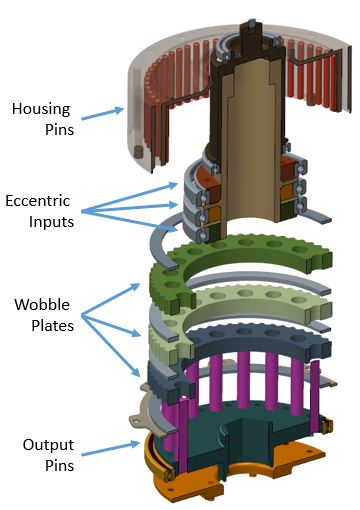
\includegraphics[width=0.7\linewidth]{fig/exploded_labeled}
   \caption{Exploded view of the cycloidal reducer.
   Three wobble plates are driven by the input shaft with 120\textdegree\ offsets.
   The ring pins are are free pins inserted in the housing.
   The output has pins run through all three wobble plates to harness the counter-rotation for the drive output.}
   \label{cycloid_exploded}
\end{figure}

The stress calculations and trading of overall size and ratio led to a necessary plate thickness of 2.38cm (0.9375in).
Instead of a single large plate, three wobble plates were selected to split the load on the central input shaft across three bearings as well as to build in natural balance for the actuator.
If a single plate is used, a counterbalance must be added to avoid substantial vibration.
In this case, the three plates were offset 120\textdegree\ to balance these loads and vibration.
This adds stack height to the system to allow separation between the plates.
This arrangement allows the large design loads to be able to be handled by the system.
The exploded view of this design can be seen in Fig \ref{cycloid_exploded}.

The actuator uses a Parker Frameless Kit Motor, model K089200-7Y with no hall effect sensors and is commutated using a Renishaw RM-44 magnetic incremental and absolute position sensor.
The final reduction is 59:1 followed by the final 5:1 output gear.
The system is commutated using the delta hysteresis commutation scheme and PI velocity control was implemented to maintain constant motor speeds \cite{ref:electric_machines}.


%\begin{figure}[!b]
   \centering
   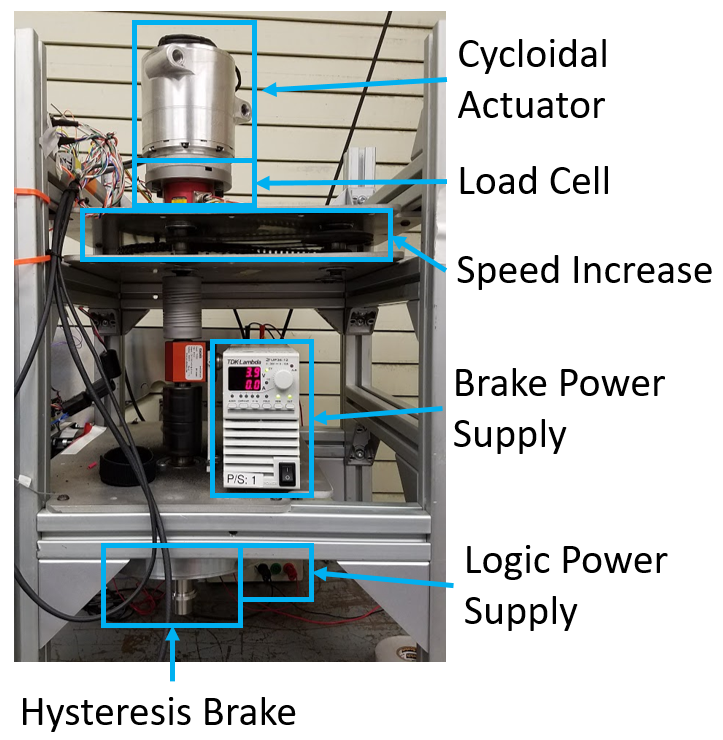
\includegraphics[width=0.75\linewidth]{fig/test_stand}
   \caption{Experimental Test Setup.
   The cycloid actuator is mounted to structure via the load cell.
   There is a speed increase so the brake can generate enough torque on the system.
   Not pictured is the controlling computer, motor driver, and high voltage supply.}
   \label{test_setup}
\end{figure}

The intent of testing the cycloidal drive is to experimentally determine and compare the in-use efficiency results to the published performance data for a comparable harmonic drive.
To accomplish this, the actuator was mounted to a Futek TF600 5000inlb load cell to measure output torque of the actuator.
The load cell signal was collected through a analog to digital converter and converted to standard units on the motor driver.
A verification of torque readings was completed using a calibrated torque wrench to ensure accuracy of the conversion.
Load was regulated by a Magtrol HB-1750 hysteresis brake.
A 36:1 speed increase was added via three chain stages between the output of the actuator and the hysteresis brake to achieve the desired applied loads.
The hysteresis brake was powered using a separate 24V Lambda-TDK power supply that was controlled through a RS-485 communication link to the test computer.
NASA's 'turbodriver' motor driver was used for commanding motor currents.
The motor driver was powered by a TDK-Lambda 12V supply for logic power and a TDK-Lambda 150V and 5A supply for high voltage power.
A hysteresis current controller was used on the motor drive to accurately provide torque producing current to the motor.
The motor driver monitored the actuator power by measuring torque from the load cell and speed with an incremental encoder located at the actuator motor shaft.
The test computer monitored the high voltage supply and recorded voltage and current to determine input power to the system and recieved data from the motor driver to calculate output power.
The test setup is shown in Fig \ref{test_setup}.

Due to the tightly integrated actuator design, the motor and cycloid cannot be separated to purely isolate the losses in the cycloid.
The efficiency map of the motor over its torque and speed range was provided by Parker Motors.
For calculation purposes, this table is used as a lookup table for efficiency of the motor given the current motor velocity and rms input current.
While this does generate a level of uncertainty in the data, these motors are mass manufactured and defects are assumed to be small.
The error in the motor efficiency map is assumed to be small and would not influence the perceived trends and results.
Power losses in the motor driver were also taken into consideration by calculating power losses in the IGBT that drives the motor.
Instantaneous current draw and a switching frequency of 12 kHz were used for the calculation, neglecting small leakage losses \cite{ref:IGBTPower}.

\begin{figure}[!b]
   \centering
   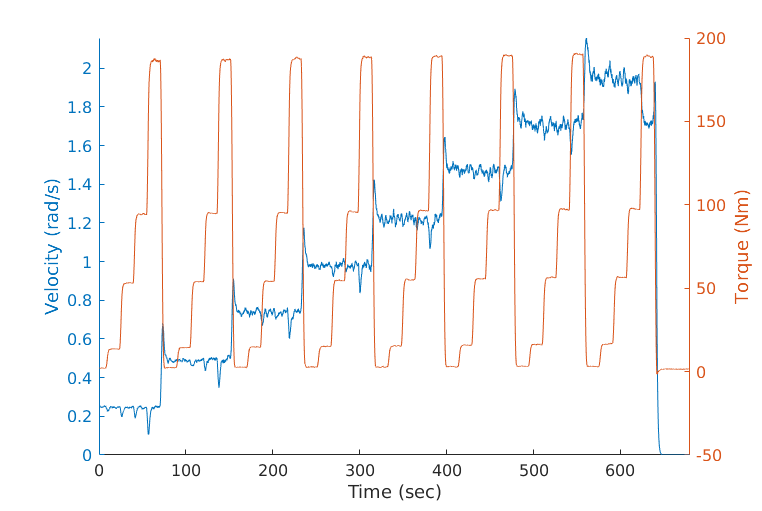
\includegraphics[width=\linewidth]{fig/eff_test_profile_v4}
   \caption{Testing profile for efficiency.
   At each speed step, torque is ramped up through five different levels, then the speed is increased.
   At the last step, the maximum of the supply was reached so motor velocity dropped.}
   \label{eff_profile}
\end{figure}

The system was tested in two separate ways, an efficiency cycle and a long term drive cycle.
The efficiency cycle test was run after the long term drive cycle to ensure steady state performance before cycling through a set of velocities and torques.
The actuator is subjected to eight velocity steps increasing 0.25 rad/s each time.
In each velocity step, the torque is ramped up and maintained for 15 seconds at values of 1Nm, 15Nm, 52Nm, 94Nm, and 189Nm.
This testing profile can be seen in Fig \ref{eff_profile}.
The long term drive cycle was run continuously each day for 6 to 12 hours with the duty cycles shown in Table \ref{table_2}.
The total runtime of the system, not including the initial checkout and verification of the actuator, has been 111 hours.

\begin{table}[h]
  \vskip0.2cm
  \caption{Long Run Drive Cycle}
  \label{table_2}
  \begin{center}
    \vskip-0.2cm
    \begin{tabular}{|c||c||c|}
    \hline
    Time (s) & Velocity (rad/s) & Torque (Nm)\\
    \hline
    150 & 1.0 & 0.0\\
    \hline
    150 & -1.0 & 0.0\\
    \hline
    60 & 0.5 & 26.0\\
    \hline
    60 & -0.5 & 26.0\\
    \hline
    150 & 1.5 & 10.0\\
    \hline
    150 & -1.5 & 10.0\\
    \hline
    30 & 1.0 & 50.0\\
    \hline
    30 & -1.0 & 50.0\\
    \hline
    300 & 0.5 & 18.0\\
    \hline
    300 & -0.5 & 18.0\\
    \hline
    \end{tabular}
  \end{center}
\end{table}

It should be noted that the actuator was used briefly in the robot validation after initial development and construction of the prototype wheel module.
The total time of use was approximately three hours.
Afterwards, it was removed from the wheel module and subjected to the characterization that is discussed in this work.
The motor has a continuous current rating of 4.3 A\textsubscript{rms} and a peak rating of 15A\textsubscript{rms}.
The actuator was designed to be liquid cooled to allow operations above the continuous values, but this could not be achieved during testing.
For long duration testing, the torque values were decreased to avoid thermal issues.
The motor was tested to approximately 6A\textsubscript{rms} during efficiency testing due to the limit of the power supply.
Also, the motor driver's rated limits are 150V, therefore the actuator's maximum rated speeds could not be tested.
The nominal cycle of the actuator as seen in Fig \ref{duty_cycle} is still achievable and has been tested.

\begin{figure*}[t]
   \centering
   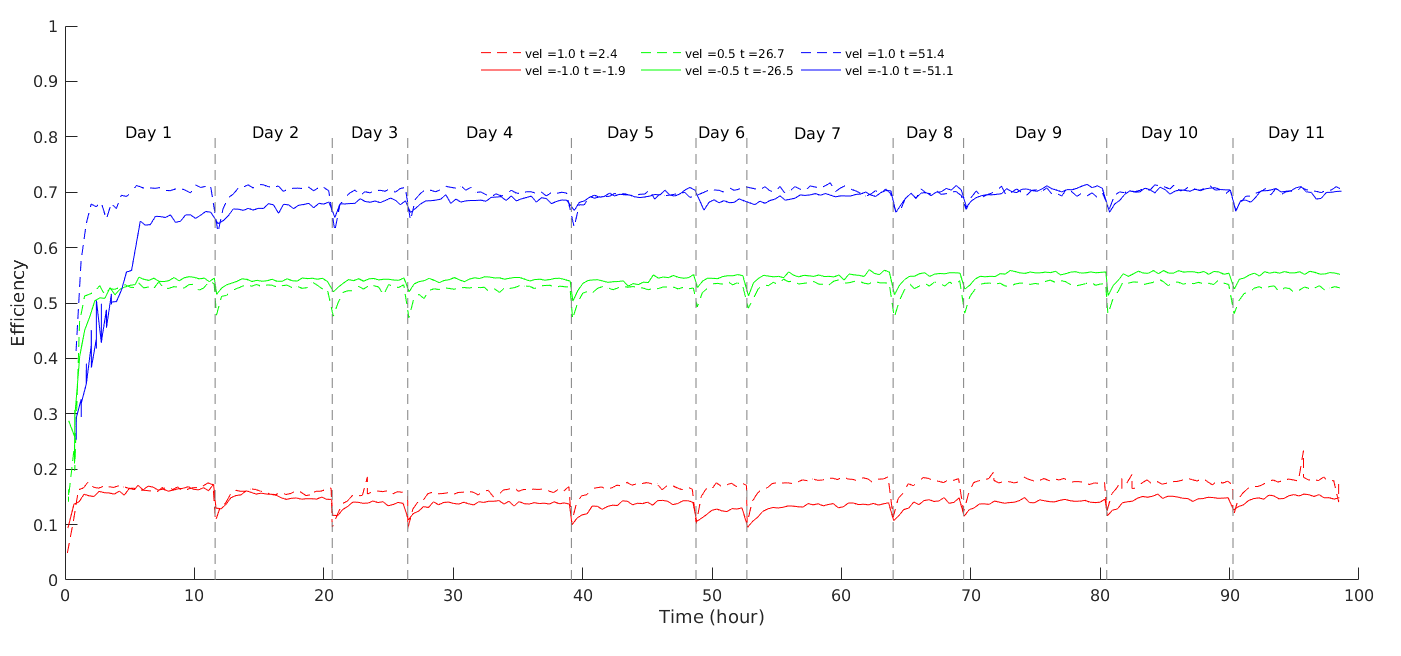
\includegraphics[width=\linewidth]{fig/long_run_plot_v4}
   \caption{Efficiency over time for three different speed/torque profiles during the drive cycle.
   The forward motion can be seen with the dotted line, reverse with the solid line.
   At the onset of testing, visible efficiency gains are made.
   As each day begins, there is a clear warm-up period before steady state.
   }
   \label{long_run}
\end{figure*}


%
\begin{figure*}[t]
   \centering
   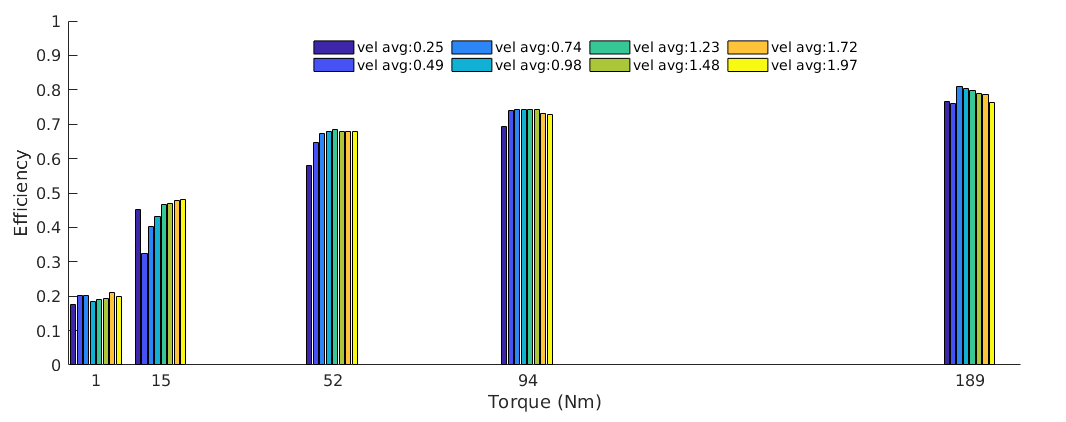
\includegraphics[width=0.8\linewidth]{fig/eff_test_bar_plot_v3}
   \caption{Grouping of average efficiencies at each torque step.
   Efficiency depends heavily on torque, and slightly on speed.}
   \label{eff_results}
\end{figure*}

Duty cycle testing was performed first on the actuator.
These tests were done at lower torques to prevent the motor from overheating to allow extended duration testing.
The total test time prior to these duty cycle tests was approximately 5.2 hours to bring up and check out the actuator testbed system.
Once this checkout was complete, the 100 hours of duty cycle testing were conducted over the course of 11 days with the drive cycle presented in Table \ref{table_2}.
Three of the torque/speed combinations in forward and reverse are plotted on Fig \ref{long_run} to show the general characteristic trends seen in actuator performance.

After this duty cycle testing to ensure the actuator had sufficiently broken-in and achieved steady state performance, as evident by Fig \ref{long_run}, the pure efficiency cycles were run.
A profile of speeds and torques (see Fig \ref{eff_profile} were run on the actuator to show the relationship between speed, torque, and efficiency.
This profile was run three times and the results at each torque and speed combination were averaged (see Fig \ref{eff_results}.

%\include{ref/icra/dicsussion}
%The aim of this work was to determine the in-use characteristics of a cycloidal drive designed for a robotic application through an extended break-in test and efficiency testing. Through the work, this study demonstrates a cycloidal actuator with a ratio of 59:1 and three phased cycloid disks that achieves a maximum efficiency of 81\% and does not show a constant efficiency through its torque profile as suggested by previous sources.
This research shows that these drives efficiencies behave very similarly to other typical reduction drives for similar applications like Harmonic Drives and Planetary gears.
This actuator compares closely to its Harmonic Drive counterpart in efficiency performance.
If backlash is acceptable in the system, a cycloidal drive has the distinct advantage of being customized into the housing using simple manufacturing techniques allowing tighter integration into a robotic system as well as a potential 2x specific torque gain.
While the efficiency and load capacity may be higher when using rolling elements for the input and output pins, this research shows that efficiencies in a similar range to other high reduction drives can be achieved when these heavy and large rolling elements are not used.
An item of interest that has not been characterized by the community is the lifetime characteristics of this cycloid design style and this is left by the authors for future work.
Cycloidal drives of this design style are quite comparable to similar use-case drives and should be considered in high reduction applications.


%The authors would like to thank the original actuator designer, Mason Markee, for his support in the testing and research of this system.  

\appendix


\bibliographystyle{ieeetr}
\bibliography{bib/thesisBib}

\end{document}
